\documentclass[a4paper,13pt,3p,twoside]{report}
\usepackage{header/packages}


% ===================================================

% \renewcommand{\bibname}{Danh_sach_tai_lieu_tham_khao} 


\addbibresource{reference.bib} % chèn file chứa danh mục tài liệu tham khảo vào 

\include{lstlisting} % Phần này cho phép chèn code và formatting code như C, C++, Python

\makeglossaries
% \makenoidxglossaries

% Danh mục thuật ngữ và từ viết tắt
% \makeglossaries	
% \makenoidxglossaries
% \glsdisablehyper

% Danh mục thuật ngữ


\newglossaryentry{lfsr}{
    type=\acronymtype,
    name={LFSR},
    description={an algorithm to generate a de Bruijn sequence using a linear function (Linear feedback shift register)},
    first = {Linear feedback shift register}
}

\newglossaryentry{fkm}{
    type=\acronymtype,
    name={FKM},
    description={Algorithm of Fredricksen, Kessler and Maiorana to generate granddaddy sequence},
}

\newglossaryentry{qkd}{
    type=\acronymtype,
    name={QKD},
    description={a secure communication method involving components of quantum mechanics for exchanging encryption keys (Quantum key distribution)},
    first = {Quantum key distribution}
}

\newglossaryentry{HdB}{
    type=\acronymtype,
    name={HdB},
    description={de Bruijn sequences encoded with a beacon model, on-on is $1$ and on-off is $0$ (Hybrid de Bruijn sequence)},
    first = {Hybrid de Bruijn}
}

\newglossaryentry{dBTS}{
    type=\acronymtype,
    name={dBTS},
    description={a timing and synchronization system using Hybrid de Bruijn code (de Bruijn based Timing and Synchronization system)},
    first = {de Bruijn based timing and synchronization system}
}

\newglossaryentry{RdB}{
    type =\acronymtype,
    name={RdB},
    description={a sequence that is the combination of positioning sequence and run length sequence (Run length limited de Bruijn sequence)},
    first = {Run length limited de Bruijn}
}

\newglossaryentry{RLL}{
    type =\acronymtype,
    name ={RLL},
    description={a line coding technique that is used to send arbitrary data over a communications channel with bandwidth limits (Run length limited)},
    first = {Run length limited}
}

\newglossaryentry{rhs}{
    type =\acronymtype,
    name ={RHS},
    description={Right hand side of a specific equation (Right Hand Side)},
}

\newglossaryentry{lhs}{
    type =\acronymtype,
    name ={LHS},
    description={Left hand side of a specific equation (Left Hand Side)},
}

% ===================================================


\fancypagestyle{plain}{%
\fancyhf{} % clear all header and footer fields
\fancyfoot[RO,RE]{\thepage} %RO=right odd, RE=right even
\renewcommand{\headrulewidth}{0pt}
\renewcommand{\footrulewidth}{0pt}}

\setlength{\headheight}{10pt}

\def \TITLE{GRADUATION THESIS}
\def \AUTHOR{Trần Văn A}

% ===================================================
\titleformat{\chapter}[hang]{\centering\bfseries}{CHAPTER \thechapter.\ }{0pt}{}[]

\titleformat 
    {\chapter} % command
    [hang] % shape
    {\centering\bfseries} % format
    {CHAPTER \thechapter.\ } % label
    {0pt} %sep
    {} % before
    [] % after
\titlespacing*{\chapter}{0pt}{-20pt}{20pt}

\titleformat
    {\section} % command
    [hang] % shape
    {\bfseries} % format
    {\thechapter.\arabic{section}\ \ \ \ } % label
    {0pt} %sep
    {} % before
    [] % after
\titlespacing{\section}{0pt}{\parskip}{0.5\parskip}

\titleformat
    {\subsection} % command
    [hang] % shape
    {\bfseries} % format
    {\thechapter.\arabic{section}.\arabic{subsection}\ \ \ \ } % label
    {0pt} %sep
    {} % before
    [] % after
\titlespacing{\subsection}{30pt}{\parskip}{0.5\parskip}

\renewcommand\thesubsubsection{\alph{subsubsection}}
\titleformat
    {\subsubsection} % command
    [hang] % shape
    {\bfseries} % format
    {\alph{subsubsection}, \ } % label
    {0pt} %sep
    {} % before
    [] % after
\titlespacing{\subsubsection}{50pt}{\parskip}{0.5\parskip}

% \newcommand{\titlesize}{\fontsize{18pt}{23pt}\selectfont}
% \newcommand{\subtitlesize}{\fontsize{16pt}{21pt}\selectfont}
% \titleclass{\part}{top}
% \titleformat{\part}[display]
%   {\normalfont\huge\bfseries}{\centering}{20pt}{\Huge\centering}
% \titlespacing{\part}{0pt}{em}{1em}
% \titlespacing{\section}{0pt}{\parskip}{0.5\parskip}
% \titlespacing{\subsection}{0pt}{\parskip}{0.5\parskip}
% \titlespacing{\subsubsection}{0pt}{\parskip}{0.5\parskip}



% ===================================================


\usepackage{hyperref}
\hypersetup{pdfborder = {0 0 0}}
\hypersetup{pdftitle={\TITLE},
	pdfauthor={\AUTHOR}}
	
\usepackage[all]{hypcap} % Cho phép tham chiếu chính xác đến hình ảnh và bảng biểu

\graphicspath{{figures/}{../figures/}} % Thư mục chứa các hình ảnh

\counterwithin{figure}{chapter} % Đánh số hình ảnh kèm theo chapter. Ví dụ: Hình 1.1, 1.2,..

\title{\bf \TITLE}
\author{\AUTHOR}

\setcounter{secnumdepth}{3} % Cho phép subsubsection trong report
% \setcounter{tocdepth}{3} % Chèn subsubsection vào bảng mục lục

\theoremstyle{definition}

\onehalfspacing
\setlength{\parskip}{6pt}
\setlength{\parindent}{15pt}


\newtheorem{theorem}{Theorem$\!$}
\newcommand{\bigCI}{\mathrel{\text{\scalebox{1.07}{$\perp\mkern-10mu\perp$}}}}
\newcommand{\cons}{{\textrm{cons}}}
\newcommand{\curv}{{\textrm{curv}}}
\newcommand{\cpc}{{\textrm{cpc}}}
\newcommand{\eps}{\epsilon}
\newtheorem{lemma}{Lemma}
\newtheorem{definition}{Definition}
\newtheorem{construction}{Construction}
\newtheorem{conjecture}{Conjecture}
\newtheorem{claim}{Claim}
\newtheorem{example}{Example}[chapter] % Định nghĩa môi trường ví dụ
\newtheorem{prop}{Proposition}
%---> Calligraphy letters -----------------

\newcommand{\cA}{{\cal A}}
\newcommand{\cB}{{\cal B}}
\newcommand{\cC}{{\cal C}}
\newcommand{\cD}{{\cal D}}
\newcommand{\cE}{{\cal E}}
\newcommand{\cF}{{\cal F}}
\newcommand{\cG}{{\cal G}}
\newcommand{\cH}{{\cal H}}
\newcommand{\cI}{{\cal I}}
\newcommand{\cJ}{{\cal J}}
\newcommand{\cK}{{\cal K}}
\newcommand{\cL}{{\cal L}}
\newcommand{\cM}{{\cal M}}
\newcommand{\cN}{{\cal N}}
\newcommand{\cO}{{\cal O}}
\newcommand{\cP}{{\cal P}}
\newcommand{\cQ}{{\cal Q}}
\newcommand{\cR}{{\cal R}}
\newcommand{\cS}{{\cal S}}
\newcommand{\cT}{{\cal T}}
\newcommand{\cU}{{\cal U}}
\newcommand{\cV}{{\cal V}}
\newcommand{\cW}{{\cal W}}
\newcommand{\cX}{{\cal X}}
\newcommand{\cY}{{\cal Y}}
\newcommand{\cZ}{{\cal Z}}
\newcommand{\A}{\mathcal A}

\newcommand{\cWC}{{\cal WC}}
%---> Script letters -----------------

\newcommand{\sA}{\script{A}}
\newcommand{\sB}{\script{B}}
\newcommand{\sC}{\script{C}}
\newcommand{\sD}{\script{D}}
\newcommand{\sE}{\script{E}}
\newcommand{\sF}{\script{F}}
\newcommand{\sG}{\script{G}}
\newcommand{\sH}{\script{H}}
\newcommand{\sI}{\script{I}}
\newcommand{\sJ}{\script{J}}
\newcommand{\sK}{\script{K}}
\newcommand{\sL}{\script{L}}
\newcommand{\sM}{\script{M}}
\newcommand{\sN}{\script{N}}
\newcommand{\sO}{\script{O}}
\newcommand{\sP}{\script{P}}
\newcommand{\sQ}{\script{Q}}
\newcommand{\sR}{\script{R}}
\newcommand{\sS}{\script{S}}
\newcommand{\sT}{\script{T}}
\newcommand{\sU}{\script{U}}
\newcommand{\sV}{\script{V}}
\newcommand{\sW}{\script{W}}
\newcommand{\sX}{\script{X}}
\newcommand{\sY}{\script{Y}}
\newcommand{\sZ}{\script{Z}}


%---> Bold letters -----------------

\newcommand{\bfa}{{\boldsymbol a}}
\newcommand{\bfb}{{\boldsymbol b}}
\newcommand{\bfc}{{\boldsymbol c}}
\newcommand{\bfd}{{\boldsymbol d}}
\newcommand{\bfe}{{\boldsymbol e}}
\newcommand{\bff}{{\boldsymbol f}}
\newcommand{\bfg}{{\boldsymbol g}}
\newcommand{\bfh}{{\boldsymbol h}}
\newcommand{\bfi}{{\boldsymbol i}}
\newcommand{\bfj}{{\boldsymbol j}}
\newcommand{\bfk}{{\boldsymbol k}}
\newcommand{\bfl}{{\boldsymbol l}}
\newcommand{\bfm}{{\boldsymbol m}}
\newcommand{\bfn}{{\boldsymbol n}}
\newcommand{\bfo}{{\boldsymbol o}}
\newcommand{\bfp}{{\boldsymbol p}}
\newcommand{\bfq}{{\boldsymbol q}}
\newcommand{\bfr}{{\boldsymbol r}}
\newcommand{\bfs}{{\boldsymbol s}}
\newcommand{\bft}{{\boldsymbol t}}
\newcommand{\bfu}{{\boldsymbol u}}
\newcommand{\bfv}{{\boldsymbol v}}
\newcommand{\bfw}{{\boldsymbol w}}
\newcommand{\bfx}{{\boldsymbol x}}
\newcommand{\bfy}{{\boldsymbol y}}
\newcommand{\bfz}{{\boldsymbol z}}
\newcommand{\bfA}{{\mathbf A}}
\newcommand{\bfB}{{\mathbf B}}
\newcommand{\bfC}{{\mathbf C}}
\newcommand{\bfD}{{\mathbf D}}
\newcommand{\bfE}{{\mathbf E}}
\newcommand{\bfF}{{\mathbf F}}
\newcommand{\bfG}{{\mathbf G}}
\newcommand{\bfH}{{\mathbf H}}
\newcommand{\bfI}{{\mathbf I}}
\newcommand{\bfJ}{{\mathbf J}}
\newcommand{\bfK}{{\mathbf K}}
\newcommand{\bfL}{{\mathbf L}}
\newcommand{\bfM}{{\mathbf M}}
\newcommand{\bfN}{{\mathbf N}}
\newcommand{\bfO}{{\mathbf O}}
\newcommand{\bfP}{{\mathbf P}}
\newcommand{\bfQ}{{\mathbf Q}}
\newcommand{\bfR}{{\mathbf R}}
\newcommand{\bfS}{{\mathbf S}}
\newcommand{\bfT}{{\mathbf T}}
\newcommand{\bfU}{{\mathbf U}}
\newcommand{\bfV}{{\mathbf V}}
\newcommand{\bfW}{{\mathbf W}}
\newcommand{\bfX}{{\mathbf X}}
\newcommand{\bfY}{{\mathbf Y}}
\newcommand{\bfZ}{{\mathbf Z}}

%---> Changing style of inequalities ------

\renewcommand{\le}{\leqslant}
\renewcommand{\leq}{\leqslant}
\renewcommand{\ge}{\geqslant}
\renewcommand{\geq}{\geqslant}

\newcommand{\card}[1]{\left \lvert #1 \right \rvert}



\newcommand\inlineeqno{\stepcounter{equation}\ (\theequation)}

% % Change citation commands to be more like old ICML styles
% \newcommand{\yrcite}[1]{\citeyearpar{#1}}
% \renewcommand{\cite}[1]{\citep{#1}}

% % modification to natbib citations
% \setcitestyle{authoryear,round,citesep={;},aysep={,},yysep={;}}


% ===================================================

{\renewcommand{\bibname}{References}}

% =========================== BODY ===============
\begin{document}
% \newgeometry{top=2cm, bottom=2cm, left=2cm, right=2cm}
\subfile{Cover} % Phần bìa
% \restoregeometry

% ===================================================
\pagestyle{empty} % Header và footer rỗng
%\newpage
%\pagenumbering{gobble} % Xóa page numbering ở cuối trang
%\subfile{chapters/0_1_subject.tex}

% \pagestyle{empty} % Header và footer rỗng
\newpage
\pagenumbering{gobble} % Xóa page numbering ở cuối trang
% \subfile{Chapter/0_2_Acknowledgment.tex}
\pagenumbering{roman}

\begin{center}
    \Large{\textbf{ACKNOWLEDGMENT}}\\
\end{center}
\vspace{1cm}

First and foremost, I would like to express my sincere gratitude to the subject teachers at Hanoi University of Science and Technology for their continuous guidance throughout my study, especially ones from School of Information and Communication Technology. During the past three and a half years, I have learned from them needed knowledge for pursuing later stages in my Computer Science journey.

I thankfully acknowledge the support of Prof. Huynh Thi Thanh Binh, who accepted me into MSO Lab and guided me in the first steps of my research career. My appreciation also extends to my laboratory colleagues, I'm very happy to have had the opportunity to collaborate with all of you, especially M.Sc. Tran Ba Trung, who introduced and invited me to joint work with him on our very first theoretical topic. I would also like to send my sincerity to other members of MSO Lab, Dr. Nguyen Thi My Binh, M.Sc. Nguyen Hong Ngoc, Tran Cong Dao, Tran Huy Hung and Tam Nguyen. Dr.Binh and M.Sc Ngoc supported me a lot when I first joint our lab. Brothers Dao, Hung, and Tam lent a hand to review my thesis. 

I also cherish the moment of doing my thesis under the supervision of Dr. Tran Vinh Duc. Though time is short, but his style in research inspired me so much. 

Taking my first step in doing theoretical research, I owe a great debt of gratitude to Dr. Ta Duy Hoang (ENS de Lyon) and Dr. Vu Van Khu (National University of Singapore) for training and mentoring me during the working on various problems including ones in this thesis. Without their support (both professionally and personally), it would not have been possible for this work to progress as far as it has. 

I'm also grateful to FPT Young Talent's members, especially Do Hoang Khanh, Lai Ngoc Tan, and Thanh La. I'll always remember the late night we spent together sharing our stories and our plans. I had known the way to find my answer to "Who am I going to be? How do I want to live in the next 10 years? 20 years?$\ldots?$" since that night.

In Bach Khoa Street Workout, my gratitude goes to Xuan Nam, Duc Anh, and Thanh Hai. We've trained and shared our experiences in SW, life and  work as brothers. 

My student's life must be harder without the following idiots: Phan Viet Hoang, Phi Phuc , Khanh Doan, Ng Duc Long, Tran Anh, Ba Tan, and Hong Sang. They are my best friends for the last four years.

I'm also very grateful to my aunt Hang and uncle Lich, who always look after me just like my mom and dad. 

Last but not least, this thesis is dedicated to my parents for the two decades of your love and support. I would not have come this far without your loving weight behind me.


% \pagestyle{empty} % Header và footer rỗng
\newpage
\pagenumbering{gobble} % Xóa page numbering ở cuối trang
\begin{center}
    \Large{\textbf{ABSTRACT}}\\
\end{center}
\vspace{1cm}
Satellite quantum key distribution is proposed to be an alternative method to establish intercontinental secure communication links instead of using optical fibre which is incapable of transmitting information in long distance due to their intrinsic exponential losses. However, it's very challenging to transmit faint quantum optical pulses between a satellite and the Earth because of unavoidable high channel losses. To overcome this issue, a classical channel is used along the quantum channel for the purpose of synchronization. In this channel, a positioning sequence is transmitted from the satellite to the stationary ground. To guarantee the timing jitter performance, the transmitted sequence must also avoid a long period of no pulses. This thesis designs Run length limited de Bruijn sequences which are not only the positioning sequence but are also able to avoid a number of consecutive $0$ bits. Such subjects are expected to have various applications and they also present some interesting theoretical questions in combinatorics, algorithms and coding theory. This thesis provides the first explicit formula for the maximal length of the run length limited de Bruijn sequences. Furthermore, using Lyndon words, an efficient construction of a run length limited de Bruijn sequence with the maximal length is presented. In addition, a sub-linear decoding algorithm which can locate the position of an arbitrary substring is also provided. 

% \begin{flushright}
% 	\begin{minipage}[t]{0.5\textwidth}
% 		\begin{center}
% 			\textit{Ha Noi}, xx May 2022\\[2cm]
		
% 			\textit{Student}
% 		\end{center}
% 	\end{minipage}
% \end{flushright}
% \pagebreak


% ===================================================
% \pagestyle{empty} % Header và footer rỗng
\newpage
\pagenumbering{gobble} % Xóa page numbering ở cuối trang
\renewcommand*\contentsname{TABLE OF CONTENTS}
\titlecontents{chapter}
    [0.0cm]             % left margin
    {\bfseries\vspace{0.3cm}}                  % above code
    {{\bfseries{\scshape} CHAPTER \thecontentslabel.\ }} % numbered format
    {}         % unnumbered format
    {\titlerule*[0.3pc]{.}\contentspage}         % filler-page-format, e.g dots
    
\titlecontents{section}
    [0.0cm]             % left margin
    {\vspace{0.3cm}}                  % above code
    {\thecontentslabel \ } % numbered format
    {}         % unnumbered format
    {\titlerule*[0.3pc]{.}\contentspage}         % filler-page-format, e.g dots
    
\titlecontents{subsection}
    [1.0cm]             % left margin
    {\vspace{0.3cm}}                  % above code
    {\thecontentslabel \ } % numbered format
    {}         % unnumbered format
    {\titlerule*[0.3pc]{.}\contentspage}         % filler-page-format, e.g dots

 % Tạo mục lục tự động
\addtocontents{toc}{\protect\thispagestyle{empty}}
\tableofcontents 
\thispagestyle{empty}
\cleardoublepage

\pagenumbering{roman}
%Tạo danh mục hình vẽ.
\renewcommand{\listfigurename}{LIST OF FIGURES}
{\let\oldnumberline\numberline
\renewcommand{\numberline}{Figure~\oldnumberline}
\listoffigures} 
% \phantomsection\addcontentsline{toc}{section}{\numberline {} DANH MỤC HÌNH VẼ}
\newpage


 %Tạo danh mục bảng biểu.
\renewcommand{\listtablename}{LIST OF TABLES}
{\let\oldnumberline\numberline
\renewcommand{\numberline}{Table~\oldnumberline}
\listoftables}
% \phantomsection\addcontentsline{toc}{section}{\numberline {} DANH MỤC BẢNG BIỂU}

\glsaddall 
% \renewcommand*{\glossaryname}{Danh sách thuật ngữ}
\renewcommand*{\acronymname}{LIST OF ABBREVIATIONS}
\renewcommand*{\entryname}{Abbreviation}
\renewcommand*{\descriptionname}{Definition}
\printglossaries

\chapter*{Notation Table} 
% \begin{table}[htbp]
%  \centering
\begin{center}
    \begin{tabular}{| m{2.5cm} | m{9cm} |}
     	\hline
     	\textbf{Notation} &\textbf{ Meaning}\\
     	\hline
     	$\Sigma_{q}$ & alphabet of size $q$, $\Sigma_{q}=(0,1,2,\ldots,q-1)$  \\  \hline
     	$\bfx\in\Sigma^{n}$ & binary sequence $\bfx$ of length $n$ over alphabet $\Sigma$ \\ \hline
     	$0^{i}$ ($1^{i}$) & concatenation of $i$ symbols $0$ ($1)$ \\ \hline
     	$W(n,s)$ & set of all sequences of length $n$ containing at most $s$ consecutive bits $0$\\  \hline
     	$\text{\L}_{n}$ & set of all Lyndon words of length $n$ \\ \hline
     	$\text{\L}^{(n)}$ & set of all Lyndon words whose length are divisors of $n$ \\ \hline
     	$\langle\bfx\rangle$ & minimal rotation of sequence $\bfx$ \\ \hline
     	$G_{k}$ & de Bruijn graph of order $k$ \\  \hline
     	$G_{k,s} = (V^{k-1,s},E^{k,s})$ & $(k,s)$-RdB graph with vertex set $V^{k-1,s}$, edges set $E^{k,s}$  \\  \hline
     	$V^{k-1,s}_{i,j}$ & set of all vertices in $G_{k,s}$ satisfying the first $i+1$ letters are $(0,0,\ldots,0,1)$ and the last $j+1$ letters are $(1,0,0,\ldots,0)$ \\  \hline
     	$\ell(G_{k,s})$ & length of the longest simple path in $G_{k,s}$ \\ \hline
     	$N(k,s)$ & length of the longest $(k,s)$-RdB sequence \\ \hline
     	$\mathbb{U}(k,s)$ & upper bound for the length of the longest simple path in $G_{k,s}$ \\ \hline
     	$\mathcal{U}(k,s)$ & upper bound for the length of the longest $(k,s)$-RdB sequence \\ \hline
     	
     \end{tabular}   
\end{center}
 
% \end{table}

% \phantomsection\addcontentsline{toc}{section}{\numberline {} DANH MỤC THUẬT NGỮ VÀ TỪ VIẾT TẮT}

\renewcommand\appendixname{APPENDIX}
\renewcommand\appendixpagename{APPENDIX}
\renewcommand\appendixtocname{APPENDIX}

\renewcommand{\figurename}{Figure}
\renewcommand{\tablename}{Table}
\renewcommand{\chaptername}{CHAPTER}

% ===================================================


\newpage
\pagenumbering{arabic}

\pagestyle{fancy}
\fancyhf{}
\fancyhead[RE, LO]{\leftmark}
%\fancyhead[LE]{\rightmark}
\fancyfoot[RE, LO]{\thepage}

\chapter{INTRODUCTION}
\label{chapter:motivation}
A de Bruijn sequence, or a positioning sequence, (of order $k$) is a binary sequence in which every possible length-$k$ string appears exactly once as a substring. The uses of de Bruijn sequences have been found in various fields. Recently, a novel application of positioning sequences has been found in quantum communication by \citeauthor{zhang2021timing}. They adopt such sequences into \gls{HdB} sequences to develop a system for synchronizing in quantum channels. Though having shown advantages against other methods~\cite{zhang2021timing}, such implementation still has drawbacks and there is room for improvements. This thesis focuses on designing a new constrained de Bruijn sequence and proving its efficiency against \gls{HdB} sequence. 

Chapter \ref{chapter:motivation} first briefly introduces the \gls{qkd} protocol, along with the reasonable motivation to study the synchronization mechanisms in satellite quantum channels. Among such mechanisms, the timing and synchronization system proposed by \citeauthor{zhang2021timing} in~\cite{zhang2021timing} is analyzed to recognize its disadvantages. The main results of this thesis, which aim to improve those weaknesses, are summarized. The organization of the whole thesis is given at the end of this chapter. 

% Chapter \ref{chapter:motivation} introduces a de Bruijn based system used in Quantum communication. The drawback of this system is the inspiration for the results in this thesis. This thesis's contributions are also summarized in this chapter. 

\section{Timing and synchronization system in quantum channels}
Symmetric, public-key (asymmetric), and hash-based cryptography are fundamental pillars of modern cryptography. While  symmetric schemes and hash functions are less vulnerable to quantum attacks, the asymmetric schemes based on factoring or solving the discrete logarithm problem, for example: Rivest-Shamir-Adelman (RSA), Elliptic Curve Cryptography, are completely broken by a quantum adversary via Shor's algorithm~\cite{shor1999polynomial}. Currently deployed public key cryptosystems are used to establish a common secret key between two parties. Doing the same jobs, \gls{qkd} enables two parties to produce a shared random secret key known only to them. Moreover, \gls{qkd} is able to guarantee the security of communication links making them immune to quantum computer-based attacks~\cite{gheorghiu2019benchmarking}. 

The first invented \gls{qkd} protocols are BB84~\cite{bennett1984quantum}, and E91~\cite{ekert1992quantum}. Since 2005, \gls{qkd} has been initially implemented in real life. For example, in 2005, University of Geneva and Corning Inc used a fiber optic wire of $307$ km. In 2007, Los Alamos National Laboratory and the National Institute of Standards and Technology (NIST) used the BB84 protocol over a 148.7 km optical fiber. In 2018, Quantum Xchange launched the first quantum network in the U.S., offering $1,000$ km of fiber optic cable and 19 colocation centers along the Boston-to-Washington, D.C., corridor and metro hubs. However, due to the intrinsic exponential losses over optical fiber, the deployed \gls{qkd} systems' range is restricted to under $1000$ km. So as to establish intercontinental secure communication links, which usually requires a range over $1000$ km, satellite \gls{qkd} has been proposed as an alternative, with the pioneering Micius satellite. In these systems, the transmitter (satellite) and the receiver (optical ground station) relentless exchange information after measuring the quantum states. But transmitting faint quantum optical pulses between a satellite and the Earth is challenging due to high channel losses cause by volatility environment and rapid relative motion between two parties. 

To deal with this problem, the reliable and efficient timing and synchronization systems have been proposed in~\cite{khader2018time,duan2021survey}. In this system, a classical channel is used along with the quantum channel, because of its advantage in synchronization. Figure~\ref{fig:qkd_satellite} shows a high-level view of this schematic.

\begin{figure}[htbp]
    \centering
    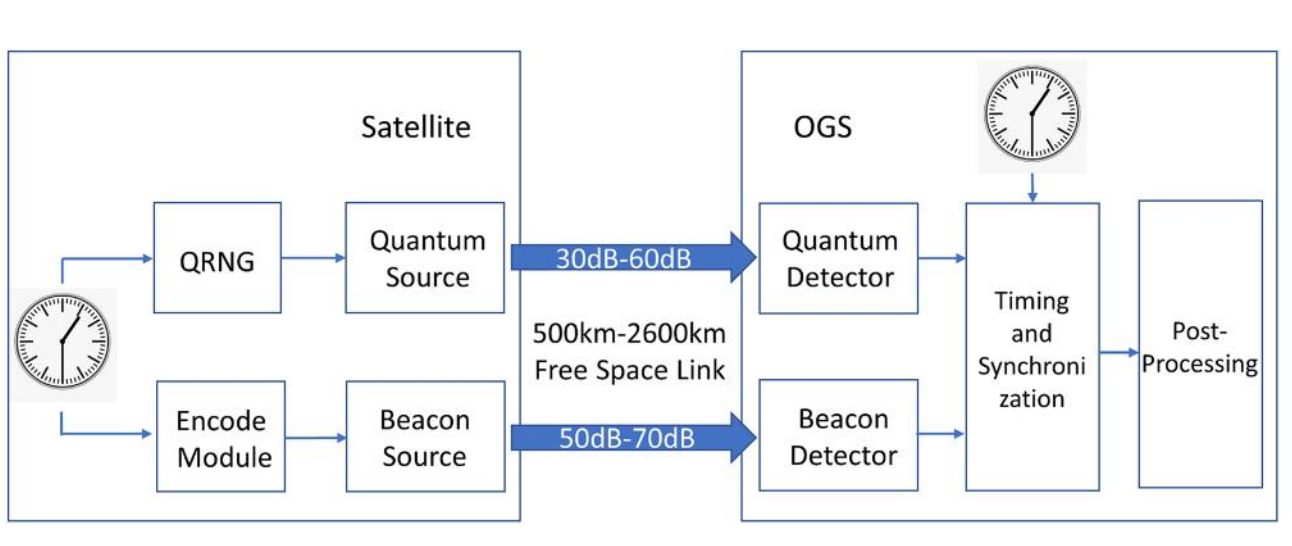
\includegraphics[scale=0.3]{fig/SatelliterQKD.png}
    \caption{High-level satellite Quantum Key Distribution timing and synchronization schematic \cite{zhang2021timing}.}
    \label{fig:qkd_satellite}
\end{figure}

Based on that concept, in~\cite{zhang2021timing}, a \gls{dBTS} is introduced using a beacon with on-off model. In this model, a de Bruijn sequence is transmitted from the satellite to the ground for synchronization. 

The encode process happens at the satellite, where it uses the \gls{lfsr} algorithm to generate a positioning sequence (of order $k$ for example). The prerequisite of finding a proper primitive polynomial is the main drawback of this encoder. 

The decode process takes place at the ground station, a look-up table is used to identify the unique position of the received sequences of length $k$. The complexity of this method is exponential.

Furthermore, in this model, a sequence of beacon pulses are used to represent a binary de Bruijn sequence. Considering the timing jitter performance, a long period of no-pulses should be forbidden. If one pulse slot is used to represent a binary bit, for example, on is 1 and off is 0, a long run of 0's in the sequence (which is a long period of no-pulses) would impact the timing jitter. In \cite{zhang2021timing}, two pulse slots are used to represent a single bit, on-on is 1 and on-off is 0, so that one can avoid two consecutive no-pulses. The transmitted sequence is called \gls{HdB}. However, the above scheme requires $2n$ pulse slots to represent a de Bruijn sequence of length $n$ and needs to receive a sub-sequence of $2 \log n$ pulse slots to locate its position. Formally, the \gls{HdB} sequence's rate is just $0.5$, where rate is a quantity that needs to be as high as possible (the definition of sequences' rate is given in section \ref{sec:rate}).

% For further illustration, the whole process, methods, and drawbacks of \gls{dBTS} system using \gls{HdB} sequence is summarized is figure \ref{fig:dBTS}
% \begin{figure}[htbp]
%     \centering
%     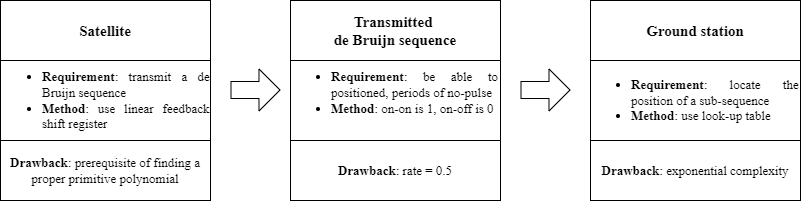
\includegraphics[scale=0.5]{fig/dBTS.png}
%     \caption{de Bruijn based timing and synchronizing system use Hybrid de Bruijn code}
%     \label{fig:dBTS}
% \end{figure}

Table \ref{tab:dBTS} summarized the process, applied methods and drawbacks of \gls{dBTS} system using \gls{HdB} sequence.
\begin{table}[htbp]
    \centering
    \caption{Timing and synchronizing system use Hybrid de Bruijn code.}
    \renewcommand{\arraystretch}{1.25}
    \resizebox{\columnwidth}{!}{
    \begin{tabular}{| p{4.1cm} | p{4.1cm}| p{4.1cm} |}
    % \begin{tabular}{|l|l|l|}
        \hline
        \textbf{Satellite} & \textbf{Transmited de Bruijn sequence} & \textbf{Ground Station} \\
        \hline \hline
        \textbf{Requirement}: transmit a de Bruijn sequence of order $k$
          &
        \textbf{Requirement}: be able to be positioned, avoid periods of no-pulse 
          &
        \textbf{Requirement}: locate the position of any length $k$ subsequence  \\
        \hline
        \textbf{Method}: use linear feedback shift register algorithm
          &
        \textbf{Method}: modulate on-on is $1$, on-off is $0$
          &
        \textbf{Method}: use look-up table \\
         \hline 
        \textbf{Drawback}: the prerequisite of finding a proper primitive polynomial 
        &
        \textbf{Drawback}: rate is $0.5$
        &
        \textbf{Drawback}: exponential complexity \\
        \hline
    \end{tabular}
    }
    \label{tab:dBTS}
    
\end{table}

% \begin{table}[htbp]
%     \centering
%     \begin{tabularx}{\textwidth} { 
%   | >{\raggedright\arraybackslash}X 
%   | >{\raggedright\arraybackslash}X 
%   | >{\raggedright\arraybackslash}X | }
%  \hline
%         \textbf{Satellite} & \textbf{Transmited de Bruijn sequence} & \textbf{Ground Station} \\
%          \hline 
%         \textbf{Requirement}: transmit a de Bruijn sequence of order $k$
%           &
%         \textbf{Requirement}: be able to be positioned, avoid periods of no-pulse 
%           &
%         \textbf{Requirement}: locate the position of any length $k$ subsequence  \\
%         \hline 
%         \textbf{Method}: use linear feedback shift register algorithm
%           &
%         \textbf{Method}: modulate on-on is $1$, on-off is $0$
%           &
%         \textbf{Method}: use look-up table \\
%          \hline 
%         \textbf{Drawback}: the prerequisite of finding a proper primitive polynomial 
%         &
%         \textbf{Drawback}: rate is $0.5$
%         &
%         \textbf{Drawback}: exponential complexity \\
%         \hline
% \end{tabularx}
%     \caption{Caption}
%     \label{tab:my_label}
% \end{table}





\section{The contributions and organization of this thesis}
This thesis aims to improve the drawback of the \gls{HdB} sequence listed above. The main task here is designing a code satisfying the constraints of \gls{dBTS} system.

\textbf{Problem Statement}: Designing a high rate sequence which is capable of positioning and avoids two consecutive symbol $0$'s.

Chapter \ref{chapter:RdB} presents the proposed sequence of this thesis, which is called Run length limited de Bruijn sequence (\gls{RdB}). The \gls{RdB} sequence is not just suitable with \gls{dBTS} system, but also have a higher rate than \gls{HdB} sequence. More precisely, rate of the longest \gls{RdB} sequence is \[\log\left(\dfrac{1+\sqrt{5}}{2}\right)\approx0.6942.\]

Chapter \ref{chapter:pro_rlldb_sequence} provides the efficient algorithm to generate one of the longest \gls{RdB} sequence. This algorithm, called an encoder, is based on the \gls{fkm}, which is the fastest method to produce a de Bruijn sequence. Moreover, to locate the position of an abitrary proper subsequence in the whole \gls{RdB} sequence, a decoder is also presented. The proposed decoder modifies the decoding algorithm found by Kociukima .et.al in \cite{kociumaka2016efficient}, which is currently the state of the art method to position a subsequence in the de Bruijn sequence, and therefore, is better than look-up table.

Beside, the \gls{RdB} sequence is even more general and adaptive. More particularly, when the constraint of forbidding pattern $00$ is relaxed, that is, a longer run of bit $0$'s is allowed, the \gls{RdB} sequence can be easily adjusted to make the its rate higher and still suits the system. 

In summary, the contributions of this thesis is listed as follows:
\begin{itemize}
    \item Proposing a new kind of sequence (\gls{RdB}), more efficient (higher rate, more general and adaptive) than \gls{HdB} sequences.
    \item Determining the length of the longest \gls{RdB} sequence.
    \item Providing fast encoder and decoder based on state of the art algorithms.
\end{itemize}

% Chương này có độ dài không quá 10 trang. Chương này sinh viên trình bày về phân tích rõ ngữ cảnh bài toán cũng như các kết quả nghiên cứu tương tự. Đồng thời, sinh viên có thể trình bày thêm về các kiến thức nền tảng.

% \section{Scope of Research}
% \ldots

% \section{Related Works}
% Trong phần này sinh viên trình bày các nghiên cứu liên quan (related work), chú ý phân tích rõ những ưu nhược điểm của chúng. Từ đó, nêu bật lên động lực để thực hiện nghiên cứu của đồ án này.


% \section{Tên của kiến thức nền tảng số 1}
% Tiêu đề và nội dung của chương này sẽ thay đổi tuỳ thuộc vào từng đồ án. Chú ý trình bày những kiến thức có liên quan mật thiết nhất đối với đồ án của mình, Tránh trình bày lan man những kiến thức phổ thông không cần thiết. 

% \section{Tên của kiến thức nền tảng số 2}
% Tiêu đề và nội dung của chương này sẽ thay đổi tuỳ thuộc vào từng đồ án. Chú ý trình bày những kiến thức có liên quan mật thiết nhất đối với đồ án của mình, Tránh trình bày lan man những kiến thức phổ thông không cần thiết.  % Phần mở đầu

\newpage
%\pagestyle{fancy} % Áp dụng header và footer
\chapter{DE BRUIJN SEQUENCE AND ITS RELATED RESULTS}
\label{chapter:deBruijnSequences}
The first section of this chapter gives a brief introduction to Coding Theory and its applications. Also, widely used terminologies and notations in Coding are provided. Following up, the de Bruijn sequence, an attractive combinatorial object in Coding theory, and the results surround it are presented. The universal cycles, which is the generalised version of de Bruijn sequence, are also concerned. The applications of these such sequences are surveyed and provided at the end of this chapter.

\section{Coding Theory}
% \begin{itemize}
%     \item \href{https://sci-hub.st/10.1007/s12243-021-00877-5}{A novel ofine indoor acoustic synchronization protocol: experimental analysis}: Another usage of de Bruijn sequence in synchronization.
%     \item \href{http://www-groups.mcs.st-andrews.ac.uk/~pjc/talks/21pmtia/pjc_pmtia2.pdf}{Synchronizing automata, de Bruijn graphs, and applications}:
%     \item \href{https://www4.comp.polyu.edu.hk/~comp2322/Bit\%20and\%20Frame\%20Synchronization\%20Techiques.pdf#:~:text=Synchronization\%20techniques\%20will\%20guide\%20the\%20receiving\%20system\%20in,the\%20need\%20for\%20error\%20control\%20at\%20higher\%20levels.}{Bit and Frame Synchronization
% Techniques}
% \end{itemize}
% {\color{red} A field where many application of de Bruijn sequences are found}
Transmitting, storing, protecting data (and so on) are challenging problems because of various factors: noisy channels, bandwidth, inter-symbol interference, $\ldots$. Coding theory is the study of the properties of codes and their fitness that helps dealing with these issues. In academic research, codes are involved in data-transmission, data-storage, data-compression, cryptography, error-detection and correction. 

\subsection{Brief overview}\label{subsec:brief_overview}
The article, "A Mathematical Theory of Communication" of Claude Shannnon, published in 1948, was considered to mark the birth of Coding Theory. In his work, Shannon showed that when a noisy communication channel is given, he defined a number, called the capacity of the channel, such that reliable communication can be achieved at any rate below the channel capacity, if proper encoding and decoding techniques are used. 


In more than half a century, coding theory has seen phenomenal growth. Many codes have been well-studied and have various application in real life. For example, Reed-Solomon code is used in 3G, 4G network, Turbo code is used in 5G network. Both Turbo code and LDPC code are channel coding technique that Data modems, telephone transmission, NASA Deep Space Network use to get the bit through. 

Usually, coding is divided into \textit{source coding} and \textit{channel coding}. 

Source coding plays a role of changing the message source to a code that is suitable for transmitting through the channel. For example, ASCII code is a source coding standard converting each character to a byte of 8 bits is an example of source coding. Another way to think about source coding is to treat it as a compress-decompress process. At the transmitter, the source encoder compresses the message for the purpose of economizing on the length of the transmission. At the other end, the source decoder decompresses the received signal or sequence. The commonly used compression algorithms include Huffman code used in JPEG, MPEG, MP3 files, Lempel-Ziv code used in ZIP files,$\cdots$.

Because of physical and engineering limitations, channels are not ideal: their output may differ from their input because of noise or manufacturing defects. The transmitted message may become distorted and the receiver might not realize that the message was corrupted. Additionally, there are applications, such as magnetic and optical mass storage media, where certain patterns are not allowed to appear in the channel's bit stream. The main role of channel coding is to overcome such limitations by encoding the message again after the source coding while maintaining the channel as transparent as possible from the source and destination points of view. 

\begin{figure}
    \centering
    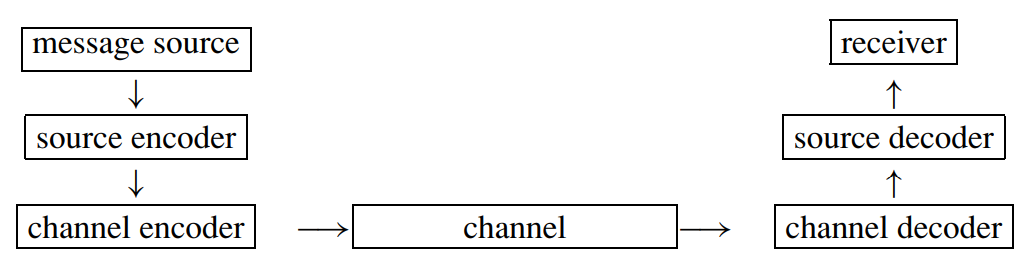
\includegraphics[scale=0.5]{fig/sourceandchannelcoding.png}
    \caption{Model of source and channel coding~\cite{ling2004coding}.}
    \label{fig:sourcechannelcoding}
\end{figure}

Section~\ref{subsec:brief_overview} has introduced to basic idea of coding theory. In the next section, this thesis provides the commonly used notations and terminologies of this research field.
\subsection{Notation and terminologies}
The most essential element of coding theory is \textbf{codeword}, which is a sequence of code symbols taken from a code alphabet
\begin{definition}[Code Alphabet]
    A code alphabet is set $\Sigma=\left\{a_{1},a_{2},\ldots,a_{q}\right\}$ of size $q$. The elements of $\Sigma$ are called code symbols, letters, and bits if $q=2$. A $q$-ary word of length $n$ over $\Sigma$ is a sequence (or string) $\bfw=w_{1}w_{2}\ldots w_{n}\in\Sigma^{n}$ with each $w_{i}\in\Sigma$ for all $i$. 
\end{definition}
In practice, the size of a code alphabet is often the size of a finite field, which is the power of a prime number. Hence, for simplicity, $\Sigma$ can be treated as a set of the first $q$ non negative integers without ambiguity. More particularly, the notation $\Sigma={0,1,2,\ldots,q-1}$ can be used instead.
\begin{definition}[Code and Codeword]
    A $q$-ary block code $C$ over $\Sigma$ is a nonempty set $C$ of $q-ary$ words of the same length $n$. Each element of $C$ is called a codeword in $C$.
\end{definition}
The study of a code $C$ involves the following process in an example of channel coding. Suppose that $\Sigma$ and $\Sigma^{\prime}$ are finite input and output of the channel respectively. Let $\bfm$, taken out of $M$ possible information words, be a message input to the channel encoder. Through a desired channel encoder, the message $\bfm$ is mapped to a longer codeword $\bfc\in\Sigma^{n}$. The word $\bfc$ is transmitted through the channel, become $\bfy\in\Sigma^{\prime n}$. After receiving $\bfy$, the role of the channel decoder is to produce codeword $\hat{\bfc}$ and a decoded information word $\hat{\bfu}$, aiming to have $\bfc=\hat{\bfc}$ and $\bfu=\hat{\bfu}$. Consequently, the mapping at the channel encoder needs to be one-to-one, and the size of the code $C$ is the maximal possible number of messages, or $\card{C}=M$.

Observe that, using code $C$, it takes a sequence of length $n$ to encode a sequence of length $\log_{\card{\Sigma}}(\card{C})$. In other words, $n-\log_{\card{\Sigma}}(\card{C})$ "redundant" bits were added to the message so that the channel can achieve its goal. Accordingly, a quantity concerning this redundancy was introduced, called \textit{(information) rate}. 
\begin{definition}[Information rate]\label{def:information_rate}
    The (information) rate of a code $C$ over an alphabet of size $q$ is defined as:
    \begin{align}
        R_{C}= \dfrac{\log_{q}(\card{C})}{n}.
    \end{align}
\end{definition}

Works in coding theory, including this thesis, are interested in designing codes with high rate, along with its efficient encoder, decoder, that can be used in specific situations. 

Based on their motive or their intrinsic properties, codes are categorized into linear codes, constrained codes, error-correcting codes, error-detecting codes,$\ldots$. This thesis focus on the combination of a constrained code, run length limited, and positioning code. A brief introduction to constrained code is given in the next section.

\subsection{Constrained code}\label{subsec:constrained_code}
Constrained Code is a sub-field of Coding theory, studies to design codes satisfying given constrained. The inspiration for the research of constrained codes comes from real problems. The transmitted data needs to follow some given standards which are necessary for the code to surmount the flaw of the environment. For instance, in the CD disc storage, errors tend to occur when there is a sequence of many consecutive $0$ bits. Consequently, it's crucial to construct codes that should avoid a long sequence of $0$ bits. A famous code invented to overcome this challenge is \gls{RLL} code by Immink~\cite{immink1990runlength}. \gls{RLL} codes are defined by $2$ parameters: $d, k$, and denoted by $(d,k)$-RLL, where $d$ and $k$ are two non-negative integers such that $d\leq k$. A finite length binary sequence 
is said to satisfy the $(d,k)$-RLL constraint if its number of $0$'s between $2$ consecutive $1$ bits is at least $d$ and at most $k$.

Illustration is a convenient way to begin understanding things. In constrained code, a graph, usually called labeled graph, is a helpful visualization technique. More particularly, a labeled graph is a directed graph with its vertices and edges labeled. Vertices in labeled graph are also called states. And the start and end vertices of a directed edge are called initial and terminal states respectively. Given a state $v$, in-edges of $v$ are edges treating $v$ as terminate state. Similarly, out-edges of $v$ are edges taking $v$ as initial state. 

For example, the graph in figure~\ref{fig:d_k_RLL} represents a $(d,k)$-RLL code. It can be verified that a sequence $w$ satisfies the $(d,k)$-RLL constraint if and only if a path whose edge labeling is $w$ exists in the graph.

\begin{figure}[htbp]
    \centering
    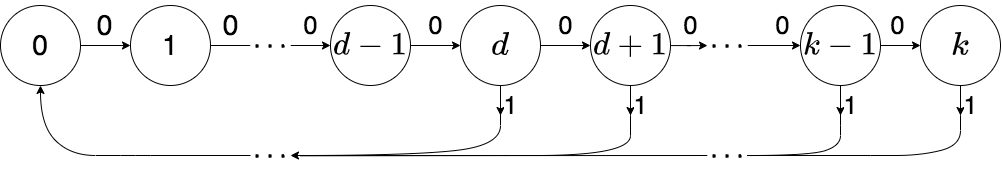
\includegraphics[scale=0.4]{fig/RLL.png}
    \caption{Graph representation of $(d,k)$-RLL code.}
    \label{fig:d_k_RLL}
\end{figure}

Labeled graphs are however more than just visualization tools. Using finite state splitting algorithm, they become encoders. In a constrained system, a very common problem is designing an encoding algorithm, which maps arbitrary user sequences into sequences obeying the constraints. Nevertheless, it's crucial to note that there are many kinds of encoders, depending on their objectives. For instance, there are encoders not taking any sequences as input, their goal are just to generate sequences satisfying given constraints. Such encoders are focused in this thesis. 

Beside constrained code, another combinatorial object drawing many attentions in coding theory is positioning code, also known by the name de Bruijn code. The formal definition of this code and its important results are presented in the next section.

% {\color{blue}
% \begin{itemize}
%     \item What is coding (def + sth from Ling San's book)
%     \item Application of coding
%     \item What are interested element in Coding (combinatorial object, encoder, decoder)
%     \item Constrained Code (Graph presentation (remember to mention in-edge, in-coming edge), Ronny)
%     \item Notation and Terminology
% \end{itemize}
% Something about error correcting, decoding ...
% }





\section{De Bruijn Sequence}
A de Bruijn sequence (of order $k$), sometimes called a positioning sequence, over an alphabet $\Sigma$, is a sequence of symbols of $\Sigma$ such that all subsequences over $\Sigma$ of length $k$ appear exactly once. This section first explains how to use a graph to represent de Bruijn sequences, and then introduces methods to generate or decode such sequences. Important results on the granddaddy, one of the most interesting de Bruijn sequences, which play a significant role in this work, are also given. 

\subsection{Graph presentation of de Bruijn sequences}

Since the first time introduced in 1946 by de Bruijn himself, the de Bruijn graph and its related sequences have been well-studied and generalized under numerous names, including positioning sequences, m-sequences, shift register sequences \cite{song2021robust,etzion1984algorithms,fredricksen1982survey,lempel1970homomorphism,cohn1977fast}. The goal of de Bruijn was to find a recursive algorithm to enumerate the number of cyclic binary sequences of length $2^k$ such that each binary $k$-tuple appears as a window of length $k$ exactly once in each sequence. 

The first results in the de Bruijn graph focused on the alphabet of size $2$. Later, in 1951, van Aardenne-Ehrenfest and de Bruijn \cite{van1951circuits} generalized the enumeration result for any arbitrary alphabet of finite size $q$, using a generalized graph for an alphabet $\Sigma$ of size $q$. 

\begin{definition}[de Bruijn graph]
    Formally, the de Bruijn Graph of order $k$, $G_{k}$ is a directed graph with $q^{k-1}$ vertices, each one is represented by a word of length $k-1$ over an alphabet $\Sigma$ with $q$ letters. A directed edge from the vertex $\bfx=(x_{0},x_{1},\ldots,x_{k-2})$ to the vertex $\bfy=(y_{1},y_{2},\ldots,y_{k-1})$, represented by the symbol $x_{k}$, where $x_{i},y_{i}\in\Sigma$, if and only if $x_{i}=y_{i}$ for all $1\leq i\leq k-2$. We call this edge $x_{k}$ the out-edge of $\bfx$, and the in-edge of $\bfy$. Progressively, the in-degree and out-degree of a vertex $\bfx$ are the numbers of in-edges and out-edges of $\bfx$ respectively.
\end{definition}  Deduced from the definition, the in-degree and out-degree of each vertex are $q$. Thus, a de Bruijn graph is an Eulerian graph. Figure \ref{fig:dB4} gives an illustration for the graph $G_{4}$.

\begin{figure}[htbp]
    \centering
    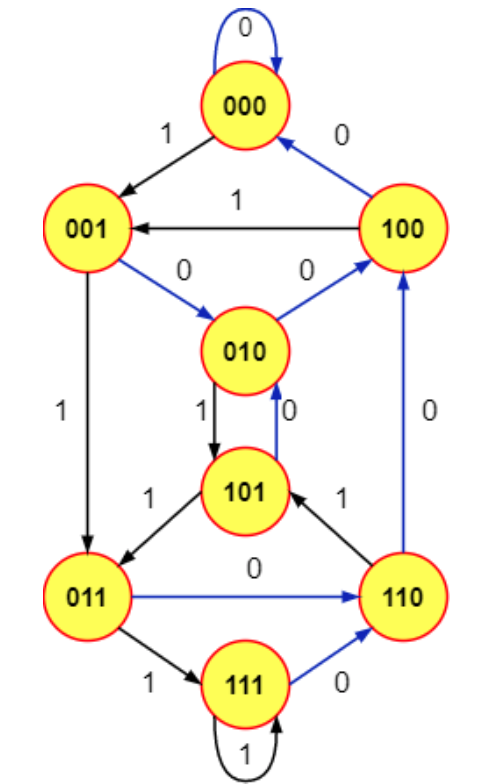
\includegraphics[scale=.3]{fig/dB4.png}
    \caption{de Bruijn graph of order $4$, $G_{4}$.}
    \label{fig:dB4}
\end{figure}

\textbf{Path}: A \textit{path} in the graph is a sequence of edges: $e_{0},e_{1},\ldots,e_{n}$ such that the terminal vertex of edge $e_{i}$ is the the initial vertex of edge $e_{i+1}$ for all $0\leq i\leq n-1$. A \textit{simple path} is a path going through each edge at most one time. Each longest simple path in a de Bruijn graph is an Eulerian cycle. A sequence formed by concatenating the symbol of each edge in the longest simple path in $G_{k}$ is called a (cyclic) de Bruijn sequence of order $k$. All the strings of length $k$ appear exactly once in each such de Bruijn sequence. The acyclic version of the de Bruijn sequence can be obtained by prepending the sequence representing the first vertex in the corresponding Eulerian cycle to the cyclic one. 

\begin{example}
    Consider an Eulerian cycle starting at vertex $000$, then the symbols representing the following edges $0,1,0,1,0,0,1,1,1,0,1,1,0,0,0$ form a de Bruijn sequence order $4$. Adding $000$ to its beginning results in an acylic one: $$0,0,0,0,1,0,1,0,0,1,1,1,0,1,1,0,0,0$$.
\end{example} 

The number of longest simple path in $G_{k}$, and also the number of de Bruijn sequences, have been proved in~\cite{van1951circuits} to be $\dfrac{q!^{q^{k-1}}}{q^{k}}$.
\begin{example}
    For $q=2,\ k=4$, there are $16$ distinct de Bruijn sequences. From figure \ref{fig:dB4}, those de Bruijn sequences are found and listed as follows:   
    \begin{center}
        \begin{tabular}{c c}
            $0000100110101111$ & $0000100111101011$ \\
            $0000101001101111$ & $0000101001111011$ \\
            $0000101100111101$ & $0000101101001111$ \\
            $0000101111001101$ & $0000101111010011$ \\
            $0000110010111101$ & $0000110100101111$ \\
            $0000110101111001$ & $0000110111100101$ \\
            $0000111100101101$ & $0000111101001011$ \\
            $0000111101011001$ & $0000111101100101$ \\
        \end{tabular}
    \end{center}
\end{example}




\subsection{Encode and decode de Bruijn sequences}
Encoding de Bruijn sequences concerns generating an arbitrary de Bruijn sequence or a de Bruijn sequence satisfying some given constraints. Finding a de Bruijn sequence is equivalent to seeking an Eulerian cycle in a de Bruijn graph. In~\cite{fleury1883deux,hierholzer1873moglichkeit}, efficient algorithms to find Eulerian cycles are presented. Especially, the approach in~\cite{fleury1883deux} can be used to generate all binary de Bruijn sequences. However, since the graph must be stored, applying such algorithms to find a positioning sequence requires exponential $O(q^k)$ space.

Besides the graph-based approach, there are other well-known methods to construct such sequences, including \gls{lfsr}, recursive methods, greedy methods, and concatenation approaches.

The idea of \gls{lfsr} is to design a feedback function $f$ mapping length $k$ strings to $\left\{0,1\right\}$. Starting with an initial length $k$ string, $f$ is repeatedly applied to the last $k$ symbols of the current string to generate the next symbol until the maximal length of a de Bruijn sequence is reached. If $f$ is linear, then, the function $F(\alpha)= \alpha f(\alpha)$ is said to be a \gls{lfsr}, where $\alpha$ is a length $k$ string. \gls{lfsr}s based on primitive polynomials generate maximal length sequences (positioning sequences) having length $2^{k}-1$ that miss only the all $0$ string. The downside of this method is that it's compulsory to find a primitive polynomial first.

De Bruijn sequences can also be constructed via recursion by applying Lempel's $D$-morphism $D:\{0,1\}^{m}\to\{0,1\}^{m-1}$ which maps a string $\alpha = \alpha_{1}\alpha_{2}\ldots\alpha_{m}$ to $\beta = \beta_{1}\beta_{2}\ldots\beta_{m-1}$, where each $b_{i} = a_{i} + a_{i+1}\ (mod\ 2)$. Nevertheless, an exponential amount of space is also required by these recursive strategies. 

Surprisingly, greedy approaches are also able to generate de Bruijn sequences. The greedy construction starts with a seed string, then repeatedly applies some greedy rule to determine the next symbol of a sequence. The algorithm stops when it is impossible to add another symbol without creating a duplicate substring of length $k$, or some termination condition is reached. The different explicit greedy rules result in different implementation greedy algorithms~\cite{martin1934problem,alhakim2010simple,fredricksen1982survey,alhakim2021revisiting}. Such constructions, however, have a major drawback: they require exponential space.

Despite many constructions being known, and even a useful survey has been given by Fredricksen~\cite{fredricksen1982survey}, things are not quite the same for the decoding problem. This problem, discovering the position within a particular sequence of any specified $k$-tuple, has been much less well studied. There are just some classical de Bruijn sequences with sub-linear decoding algorithm~\cite{mitchell1996method,tuliani2001bruijn,kociumaka2016efficient}. 

\subsection{Results on lexicographically minimal de Bruijn sequence}

The lexicographically minimal de Bruijn sequence, or \textbf{granddaddy sequence} as called by Knuth~\cite{knuth2013art}, is one the most interesting among other de Bruijn sequences. An example of granddaddy is provided in example~\ref{exp:granddaddy}.
\begin{example}[Granddaddy of order $6$]\label{exp:granddaddy}
    \[0000001000011000101000111001001011001101001111010101110110111111\]    
\end{example}
Both efficient encoder and decoder of this sequence have been found.

The encoding algorithm is actually a concatenation scheme, which is later called \gls{fkm} algorithm, the abbreviation of Fredrickesen, Kessller, and Maiorana, who discovered this strategy~\cite{fredricksen1978necklaces,fredricksen1986algorithm}. Its complexity has been proved to be constant amortized time per symbol by Frank Ruskey et.al~\cite{ruskey1992generating} in 1992.

Though its construction and the related algorithm has been found in 1978, about 40 years ago, the granddaddy's decoder has just been discovered recently in 2016 by Kociumaka, Radoszewski, and W. Rytter~\cite{kociumaka2016efficient}. Denote $\bfx$ as a granddaddy sequence of order $k$, and $v$ is a length $k$ arbitrary substring. Then the decoding algorithm, denoted by $\cD_{KRR}$, returns $\cD_{KRR}(v)$ being the one and only position of $v$ in the whole sequence $\bfx$. Kociumala et.al also proved that $\cD_{KRR}$ works in $O(k^2\log(q))$-time in the word-RAM model and $O(k^{2})$-time in unit-cost RAM model.

\section{Universal Cycles}\label{sec:universal_cycles}
A more general way to look at de Bruijn sequences is the universal cycle ($U$-cycle). 
\begin{definition}[Universal cycle]
    Given a finite set $\mathcal{T}_{k}$ of distinct of combinatorial objects of "rank $k$", an $U$-cycle of $\mathcal{T}_{k}$ is a cyclic sequence $\cU=(a_0,a_1,\ldots,a_n)$ such that $(a_{i+1},\ldots,a_{i+k})$, $0\leq i\leq n$, run through each element of $\mathcal{T}_{k}$, where index addition is performed modulo $n$.
\end{definition} 
An order $k$ binary de Bruijn sequence is eventually an $U$-cycle of the set of all length $k$ binary strings. The studies of $U$-cycle are concerned with the existence and construction of $U$-cycles for many combinatorial objects such as strings, permutations, partitions, subsets, multisets, lattice paths, vector spaces weak orders, etc~\cite{chung1992universal,horan2013universal,jackson2009research,johnson2009universal,hurlbert2009universal,jackson2009recursive}. Section~\ref{subsect:fanchung} provides results for permutations, partitions, and subsets of a set of $n$ distinct symbols, where $n$ is a positive integer. These results were first summarized by \citeauthor{chung1992universal} in~\cite{chung1992universal}.
%, for example: the set of all $n!$ permutations of $\left\{1,2,\ldots,n\right\}$, partitions of $\left\{1,2,\ldots,n\right\}$~\cite{chung1992universal}. 

\subsection{Permutations, partitions and subsets of \texorpdfstring{$n$}{n} distinct symbols}\label{subsect:fanchung}
Consider the set $S_{n}$ of all $n!$ permutations of $\left\{1,2,\ldots,n\right\}$. With each value of $n$, set $S_{n}$ may not always contain any $U$-cycles, such as $n=3$. All $6$ permutations of $\left\{1,2,3\right\}$ are $S_{3}=\left\{123,132,213,231,312,321\right\}$, and the longest cycle in $S_{3}$ one can travel is of length $4$, for instance,  $123\rightarrow231\rightarrow312\rightarrow123$, which still lacks $132, 321$. 

However, if order-isomorphism is allowed instead of requiring exact matches, $U$-cycles of $S_{n}$ exists. More precisely, an $U$-cycle $U_{n}=(a_{0},a_{1},\ldots,a_{n!-1})$, $a_{i}\in\left\{1,2,\ldots,N\right\}$, for $S_{n}$ is $n!$-tuple such that each element of $S_{n}$ is order-isomorphic to exactly one block $(a_{i+1},\ldots,a_{i+n})$, where $a_{i}=a_{j\equiv i(\mod n!)}$. Here, two $n$-tuples $\bfa=\left(a_{1},a_{2},\ldots,a_{n}\right)$ and $\bfb=\left(b_{1},b_{2},\ldots,b_{n}\right)$ are called order-isomorphic, written as $\bfa\sim\bfb$, if $a_{i}<a_{j} \Leftrightarrow b_{i}<b_{j}$ for all $0<i,j\leq n$. An example of $U$-cycle for $S_{3}$ is :
\[1\ 4\ 5\ 2\ 4 \ 3\]

By order-isomorphism, each $3$-tuple in the above $U$-cycles can be mapped into elements of $S_{3}$ as follow:
\begin{align*}
    145\sim123 \\
    452\sim231 \\
    524\sim312 \\
    243\sim132 \\
    431\sim312 \\
    314\sim213 
\end{align*}
and hence, the equivalent cycle is $123\rightarrow 231\rightarrow 312\rightarrow132\rightarrow312\rightarrow 213\rightarrow123 $. The construction of de Bruijn graphs can be imitated to construct the transition graph for $S_{n}$. Each permutation plays the role of a vertex. Their suffix of length $n-1$ is analyzed to establish its edges to other permutations. Takes the vertex $231$ of $S_{3}$ as an example. From its suffix $31$, one can go to $312$. But since order-isomorphism is accepted, and note that $31\sim21\sim32$, there are also edges connecting $231$ to $213$ and $321$. The whole transition graph of $S_{3}$ is shown in figure \ref{fig:S3_graph}.

\begin{figure}[htbp]
    \centering
    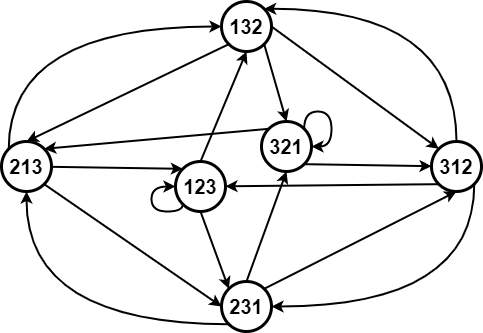
\includegraphics[scale=0.5]{fig/PermutationGraph.png}
    \caption{Transition graph of $S_{3}$.}
    \label{fig:S3_graph}
\end{figure}

It is proved that the transition graph of $S_{n}$ is Hamiltonian, and a Hamiltonian cycle in the transition graph corresponds to an $U$-cycle in $S_{n}$. Now, the key question is how to represent a $U$-cycle of an Hamiltonian cycle, like the sequence $1\ 4\ 5\ 2\ 4\ 3$ represents $123\rightarrow 231\rightarrow 312\rightarrow132\rightarrow312\rightarrow 213\rightarrow123 $. Even with $S_{3}$, is $5$ the smallest number of distinct symbols necessary for an $U$-cycle. More generally, how many distinct symbols does an $U$-cycle of $S_{n}$ use at least? 

Actually, in $S_{3}$, one can do better with $4$ symbols. For example, the sequence $1\ 4\ 2\ 3\ 4\ 2$ is the representation of a Hamiltonian cycle:
\[132\rightarrow312\rightarrow123\rightarrow231\rightarrow321\rightarrow213\rightarrow132\]

The following sequence is an example with $5$ symbols for $S_{4}$:
\[1\ 2\ 3\ 4\ 1\ 2\ 5\ 3\ 4\ 1\ 5\ 3\ 2\ 1\ 4\ 5\ 3\ 2\ 4\ 1\ 3\ 2\ 5\ 4 \]

Let $N(n)$ be the minimum number required for an $U$-cycle of $S_{n}$, it is proved that:
\[N(2)=2,\ N(3) = 4,\ N(4)=5\ \mathrm{and}\ n+1\leq N(n)\leq 6n\ \mathrm{for}\ n\geq5\]

Fan Chung believes that the equation happens at $n+1$. However, their belief remains an unsolved conjecture until now.
\begin{conjecture}
    $N(n)=n+1$.
\end{conjecture}

Constructing transition graph is also help finding $U$-cycle for the set of $P_{n}$ of partitions of the set $\left\{1,2,\ldots,n\right\}$. The partitions can be represented by sequence of length $n$ $(a_{0},a_{1},\ldots,a_{n})$, where $a_{i}=a_{j}$ indicates the $i$-th element and $j$-th element are in the same group of the partition. The transition graph of $P_{n}$ is illustrated in figure~\ref{fig:P3_graph}.

\begin{figure}[htbp]
    \centering
    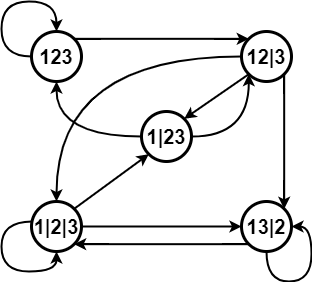
\includegraphics[scale=0.5]{fig/partitions.png}
    \caption{Transition graph of $P_{3}$.}
    \label{fig:P3_graph}
\end{figure}

The transition graph of $P_{n}$ is proved to be Hamiltonian by showing that it can be clustered to be an Eulerian graph. 

It is more challenging to study the family ${n \brack k}$ of all $k$-element subsets of a set of $n$ distinct elements $\left\{0,1,\ldots,n-1\right\}$. This thesis provides an example of an $U$-cycle for the case $n=5,k=2$:
\[1\ 3\ 2\ 5\ 4\ 2\ 1\ 5\ 3\ 4\]

The question about the condition for the existence of the universal cycle for such a family is still not answered completely. The difficulty here is that a transition graph for ${n \brack k}$ isn't able to be defined explicitly. This issue is caused by the distinguishing feature of an $k$-set. More precisely, a $k$-element subset might occur in any $k!$ possible order in the $U$-cycle, but it is only allowed to occur once. Fan Chung and Graham made a conjecture on this problem and the first person who can solve it would earn a prize awarded by the author's conjecture.

\begin{conjecture}[Fan Chung's conjecture]\label{conjecture:fanchung}
    Universal cycle for ${n \brack k}$ always exists provided $k$ divides $\dbinom{n-1}{k-1}$ and $n$ is large enough.
\end{conjecture}

It's easy to see that conjecture~\ref{conjecture:fanchung} is true for $k=1,2$. Effort on this question has just cracked completely the cases $k=3,4,5$ (with some aid of a computer), and $k=6$ whenever $n\ \mathrm{and}\ k$ are relatively prime(~\cite{hurlbert1994universal,jackson1993universal}). For $k\geq 7$, and $k=6$ when $n\ \mathrm{and}\ k$ are not relatively prime, conjecture~\ref{conjecture:fanchung} remains open. 

Besides studying the existence of $U$-cycle on different kinds of sets, designing algorithms that create universal cycles is also concerned.
\subsection{Universal cycles algorithms for other classes of sets}
There are researches focusing on using generalized the \gls{fkm} algorithm and greedy algorithm to create universal cycles for a class of sets. Moreno proved that this method works for the set of rotations of the lexicographically largest $i$ necklace~\cite{moreno2004theorem}. The aperiodic strings in the set of all $k$-ary strings of length $n$ can be generated the same way as shown by Au in~\cite{au2015generalized}. All these results are later generalized by Joe Sawada et.al in~\cite{sawada2016generalizing}. More particularly, let $\bfS$ be the set of length $n$ $k$-ary strings such that the following closure conditions are obeyed:
\begin{itemize}
    \item The set of strings $\bfS$ is closed under rotation.
    \item Its subset of necklaces is closed under replacing any suffix of length $i$ by $k^i$. 
\end{itemize}

Then, the greedy and \gls{fkm} algorithm create the lexicographically smallest universal cycle of $\bfS$. Several such classes $\bfS$ are listed in example~\ref{exp:closed_S}.

\begin{example}\label{exp:closed_S}
Recall that $\Sigma_{q}=\{1,2,3,\ldots,q\}$ is a code alphabet of size $q$, and $\Sigma_{q}^{n}$ is the set of $q$-ary sequences of length $n$ over alphabet $\Sigma$. The following sets satisfy the closure conditions for the existence of universal cycles proved by Sawada~\cite{sawada2016generalizing}.
\begin{itemize}
    \item \textbf{Minimum Sum}: $\bfS\in\Sigma_{q}^{n}$ is a set of length $n$ strings with sum over all of its symbol at least $s$, where $s$ is a given constant.
    \item \textbf{Frequency of $q$}: $\bfS\in\Sigma_{q}^{n}$ contains the strings with at least $l_{q}$ copies of $q$, where $l_{q}$ is a given constant.
    \item \textbf{Frequency of $i<q$}: $\bfS\in\Sigma_{q}^{n}$ contains the strings with at most $u_{i}$ copies of $i<q$. Here, $u_{i}$ is a given constant.
    \item \textbf{Avoiding a substring}: $\bfS\in\Sigma_{q}^{n}$ contains the strings that do not contain a given pattern $\alpha\in\Sigma_{q-1}^{m}$, for some $m\geq1$, as a cyclic substring. 
    \item \textbf{Union and Intersection}: Let $\bfS_{1}$ and $\bfS_{2}$ be $2$ set obeying the closure conditions, then both $\bfS_{1}\cup \bfS_{2}$ and $\bfS_{1}\cap \bfS_{2}$ also satisfy those conditions.
\end{itemize}
\end{example}
Note that, in example~\ref{exp:closed_S}, the union and intersection of the proper sets $\bfS$ allow to combine the previous results to create more interesting classes of sets that have universal cycles. 

Section~\ref{sec:universal_cycles} has provides different research directions and results on the universal cycle, which is a generalization of de Bruijn sequences. The applications of de Bruijn sequences and their generalizations will be presented in the next section. 


\section{Applications }
The reason why de Bruijn graph, its sequence, and their generalizations are having so much attention is due to their diverse important applications. Very soon after the formal definition of this graph was given birth, one of its first applications was found in the introduction of shift-register sequences in general and linear feed-back registers in particular~\cite{golomb19821967}. Throught out the years, these type of sequences and graphs have found a variety of applications.

In cryptography, for example, the Baltimore Hilton Inn used de Bruijn sequence to install a cipher lock system for each of its rooms in lieu of the conventional key-lock system~\cite{fredricksen1982survey}. The low-cost n-stage shift register was used to generate maximum-length pseudorandom sequences in stream cipher, though later, this method was proved to be vulnerable to known-plaintext attack~\cite{lempel1979cryptology}.

De Bruijn sequences also opened a new field of research surround its complexity. Agnes Hui Chan et.al studied the complexity and the distribution of the complexities of de Bruijn sequences~\cite{chan1982complexities}. Especially, for binary sequence with period $2^n$, they come up with a fast algorithm determining its complexity~\cite{games1983fast}. Edwin on himself analysed the structure and complexity of nonlinear binary sequence generators~\cite{key1976analysis}. Tuvi et.al studied the error linear complexity spectrum of binary sequences with period $2n$~\cite{etzion2009properties}. Also Tuvi, in his joint work with Lampel~\cite{etzion1984construction}, found a construction of de Bruijn sequence to show that the lower bound of its complexity ($2^{n-1}+n$) is attainable for all $n$.

In~\cite{lempel1985design}, A.Lampel and M.Cohn are interested in designing an universal test sequeces for VLSI (very large scale integration chip). A binary sequence is called $(s,t)$-universal, $s>t$, if when shifted through a register of length $s$, it exercises every subset of $t$ register positions. Their proposed method was concatenating a set of de Bruijn sequences of appropriate length. In~\cite{barzilai1983exhaustive}, Zeev Barzilai .et.al also demonstrated an application of de Bruijn sequence in VLSI self-testing.

There are also other applications requiring two-dimensional version of de Bruijn sequeces. And the research about two-dimensional generalization of de Bruijn sequences comes to call. One well-known version is called pseudo-random arrays. In 1976, Mac Williams and Neil Sloane~\cite{macwilliams1976pseudo} gave a simple description of pseudo-random arrays and studied several of their nice properties. In 1988, Tuvi~\cite{etzion1988constructions}, represented a new version of pseudo-random arrays to construct perfect maps. Another approach by Bruck Stein~\cite{bruckstein2012simple}, he combined a de Bruijn sequence and a half de Bruijn sequece to study it robust and self-location properties. Studies~\cite{hsieh2001decoding,morano1998structured,pages2005optimised,salvi2010state,van1994digital} used pseudo-random arrays to with applications to robust undetectable digital watermarking of two-dimensional test images, and structured light. 

More surprisingly, de Bruijn's modern applications are even combined with biology, like the genome assembly as part of DNA sequencing. For example, Chaisson et.al~\cite{chaisson2009novo} described a new tool, EULER-USR, for assembling mate-paired short reads and use it to analyze the question of whether the read length matters. Compeau et.al~\cite{compeau2011apply} represented a method using de Bruijn graph to genome assembly. In 2001, Pevzner et.al~\cite{pevzner2001new} abandoned the classical “overlap - layout - consensus” approach in favor of a new Eulerian Superpath approach, that, for the first time, resolves the problem of repeats in fragment assembly. Later on, in 2003, Yu Zhang and Michael Waterman~\cite{zhang2003eulerian}, adapted the Pevzner's method to global multiple aligment for DNA sequences. In DNA storage, Han Mao et.al~\cite{chang2017rates,kiah2016codes} studied codes and their rates for DNA sequence profiles. Their studies were based on de Brujn graph.

In some new memory technologies, mainly in racetrack memories, and other ones which can be viewed as an $l$-read channel, synchronization errors (which are shift errors known also as deletions and sticky insertions) occur. By proposing a new de Bruijn based schema, used locally-constrained de Bruijn sequence to construct such code, Chee et.al~\cite{chee2021locally} are able to increase the rate of codes which correct the synchronization errors. Locally-constrained de Bruijn sequences and codes (sets of sequences) are of interest in their own right from both practical and theoretical points of view.

Recently, in 2021, a novel application of de Bruijn sequence has been found in quantum communication. Generally, to transmit quantum information between a satellite and the ground station, a timing and synchronization system has been used. Having observed that the intrinsic properties of positioning sequence are very suitable for this system, Peide Zhang et.al~\cite{zhang2021timing} have modulated it into \gls{HdB} sequence to transmit along the quantum channel. %More details about this application are provided and clarified in the following chapter, chapter~\ref{chapter:motivation}.




% Lưu ý: Mẫu ĐATN này được thiết kế phù hợp với đồ án tốt nghiệp theo hướng nghiên cứu. Mẫu đề tài này là gợi ý tham khảo. Tuỳ từng đề tài, cấu trúc có thể thay đổi ít nhiều. Sinh viên cần tham khảo ý kiến của giáo viên hướng dẫn để đưa ra cấu trúc hợp lý nhất cho đề tài của mình. 

% Trước khi viết ĐATN, sinh viên cần đọc kỹ hướng dẫn và quy định chi tiết về cách viết ĐATN trong Phụ lục A. 

% Khi đóng quyển ĐATN, sinh viên cần lưu ý tuân thủ hướng dẫn ở phụ lục A.9

% SV cần đặc biệt lưu ý cách hành văn. Mỗi đoạn văn không được quá dài và cần có ý tứ rõ ràng, bao gồm duy nhất một ý chính và các ý phân tích bổ trợ để làm rõ hơn ý chính. Các câu văn trong đoạn phải đầy đủ chủ ngữ vị ngữ, cùng hướng đến chủ đề chung. Câu sau phải liên kết với câu trước, đoạn sau liên kết với đoạn trước. Trong văn phong khoa học, sinh viên không được dùng từ trong văn nói, không dùng các từ phóng đại, thái quá, các từ thiếu khách quan, thiên về cảm xúc, về quan điểm cá nhân như “tuyệt vời”, “cực hay”, “cực kỳ hữu ích”, v.v. Các câu văn cần được tối ưu hóa, đảm bảo rất khó để thể thêm hoặc bớt đi được dù chỉ một từ. Cách diễn đạt cần ngắn gọn, súc tích, không dài dòng.


% Chương 1 có độ dài từ 3 đến 6 trang với các nội dung sau đây


% \section{Problem Statement}
% \label{sec:dvd}
% Phần này sinh viên mô tả bài toán cần giải quyết, lý do tại sao lại chọn bài toán đó, ý nghĩa/tầm quan trọng của bài toán.

% Tiêu đề của chương này có thể để là ``đặt vấn đề'', hoặc lấy chính tên của bài toán mà sinh viên định giải quyết, ví dụ có thể đặt tiêu đề là ``Bài toán dự đoán …” 


% \section{Background and Problems of Research} 
% \label{sec:giaiphap}
% Sinh viên trước tiên cần trình bày tổng quan các kết quả của các nghiên cứu hiện nay cho bài toán giới thiệu ở phần \ref{sec:dvd}. Sau đấy, sinh viên đưa ra các hạn chế của các giải pháp hiện tại. 

% \section{Research Objectives and Conceptual Framework}
% Trong chương này, sinh viên trước hết trình bày mục tiêu của đồ án là gì, sau đấy sinh viên đề xuất định hướng giải pháp của mình. Tốt nhất là với trình bày từng giải pháp đối với mỗi vấn đề nêu ra trong chương \ref{sec:giaiphap}. 

% \section{Contributions}
% Trong phần này sinh viên liệt kê cụ thể, ngắn gọn các đóng góp của đồ án. Ví dụ: 

% Đồ án này có 3 đóng góp chính như sau:

% \begin{enumerate}
% \item Đồ án đề xuất một phương pháp tiền xử lý dữ liệu nhằm loại bỏ nhiễu và dữ liệu ngoại lai trước khi đưa vào huấn luyện mô hình.
% \item \ldots
% \item \ldots 
% \end{enumerate}

% \section{Organization of Thesis}
% Phần còn lại của báo cáo đồ án tốt nghiệp này được tổ chức như sau. 

% Chương 2 trình bày về v.v. 

% Trong Chương 3, em/tôi giới thiệu về v.v.

% Chú ý: Sinh viên cần viết mô tả thành đoạn văn đầy đủ về nội dung chương. Tuyệt đối không viết ý hay gạch đầu dòng. Chương 1 không cần mô tả trong phần này. 

% Ví dụ tham khảo mô tả chương trong phần bố cục đồ án tốt nghiệp: Chương *** trình bày đóng góp chính của đồ án, đó là một nền tảng ABC cho phép khai phá và tích hợp nhiều nguồn dữ liệu, trong đó mỗi nguồn dữ liệu lại có định dạng đặc thù riêng. Nền tảng ABC được phát triển dựa trên khái niệm DEF, là các module ngữ nghĩa trợ giúp người dùng tìm kiếm, tích hợp và hiển thị trực quan dữ liệu theo mô hình cộng tác và mô hình phân tán.  

% Chú ý: Trong phần nội dung chính, mỗi chương của đồ án nên có phần Tổng quan và Kết chương. Hai phần này đều có định dạng văn bản “Normal”, sinh viên không cần tạo định dạng riêng, ví dụ như không in đậm/in nghiêng, không đóng khung, v.v... 

% Trong phần Tổng quan của chương N, sinh viên nên có sự liên kết với chương N-1 rồi trình bày sơ qua lý do có mặt của chương N và sự cần thiết của chương này trong đồ án. Sau đó giới thiệu những vấn đề sẽ trình bày trong chương này là gì, trong các đề mục lớn nào.

% Ví dụ về phần Tổng quan: Chương 3 đã thảo luận về nguồn gốc ra đời, cơ sở lý thuyết và các nhiệm vụ chính của bài toán tích hợp dữ liệu. Chương 4 này sẽ trình bày chi tiết các công cụ tích hợp dữ liệu theo hướng tiếp cận “mashup”. Với mục đích và phạm vi của đề tài, sáu nhóm công cụ tích hợp dữ liệu chính được trình bày bao gồm: (i) nhóm công cụ ABC trong phần 4.1, (ii) nhóm công cụ DEF trong phần 4.2, nhóm công cụ GHK trong phần 4.3, v.v...

% Trong phần Kết chương, sinh viên đưa ra một số kết luận quan trọng của chương. Những vấn đề mở ra trong Tổng quan cần được tóm tắt lại nội dung và cách giải quyết/thực hiện như thế nào. Sinh viên lưu ý không viết Kết chương giống hệt Tổng quan. Sau khi đọc phần Kết chương, người đọc sẽ nắm được sơ bộ nội dung và giải pháp cho các vấn đề đã trình bày trong chương. Trong Kết chương, Sinh viên nên có thêm câu liên kết tới chương tiếp theo.

% Ví dụ về phần Kết chương: Chương này đã phân tích chi tiết sáu nhóm công cụ tích hợp dữ liệu. Nhóm công cụ ABC và DEF thích hợp với những bài toán tích hợp dữ liệu phạm vi nhỏ. Trong khi đó, nhóm công cụ GHK lại chứng tỏ thế mạnh của mình với những bài toán cần độ chính xác cao, v.v. Từ kết quả nghiên cứu và phân tích về sáu nhóm công cụ tích hợp dữ liệu này, tôi đã thực hiện phát triển phần mềm tự động bóc tách và tích hợp dữ liệu sử dụng nhóm công cụ GHK. Phần này được trình bày trong chương tiếp theo – Chương 5.



\newpage
%\pagestyle{fancy} % Áp dụng header và footer
\chapter{RUNLENGTH LIMITED DE BRUIJN SEQUENCE}
\label{chapter:RdB}
In this chapter, new constrained de Bruijn sequences are introduced. Since a de Bruijn sequence is self-located, the run length limited constraint is the only requirement remaining that this sequence needs to satisfy to be used in the \gls{dBTS} system. Therefore, combining a positioning sequence and a run length limited sequence is a natural solution. That is also how this thesis gave birth to the name: Run length limited de Bruijn sequence. Besides, just like other constrained codes, a convenient way to apprehend a code is using a labeled graph. Hence, the graph presentation of these sequences is also provided. 

\section{Run length limited de Bruijn sequence}

Let $n,k,s,q$ be some positive integers and $\Sigma_{q} = \left\{0,1,2,\ldots,q-1\right\}$ be an alphabet of size $q$. A \emph{sequence} $\bfs=\left(s_{1},s_{2},\ldots,s_{n}\right)\in\Sigma^{n}_{q}$ is over an alphabet $\Sigma$, that is, $s_{i}\in\Sigma_{q}$. This thesis only focuses on the case $q=2$ and thus drops $q$ in the notation for simplicity. Sequence $\bfs=s_{1}s_{2}\ldots s_{n}\in\Sigma^{n}$ is also written without ambiguity. The window (substring) $(s_{i},s_{i+1},\ldots,s_{j})$ is denoted by $s[i,j]$. 

Given two sequences $\bfx=x_{1}x_{2}\ldots x_{m}$ and $\bfy=y_{1}y_{2}\ldots y_{n}$, denote the concatenation of $\bfx$ and $\bfy$ to be $\bfx\bfy $ $=x_{1}x_{2}\ldots x_{m}y_{1}y_{2}\ldots y_{n}$, and denote $\bfx^{k}$ the concatenation of $k$ copies of $\bfx$. It is said that $\bfx$ is smaller than $\bfy$, denoted $\bfx<\bfy$, if there is an index $t\geq1$, such that $x_{i}=y_{i}$, $\forall i\leq t$, and $x_{t+1}<y_{t+1}$. Note that empty sequence is smaller than $0$.

\begin{definition}
    A  sequence $\bfs = (s_1,s_2,\ldots,s_n)$ is called a $s$-run length limited (RLL) sequence of length $n$ if each run of 0's in the sequence $\bfs$ has length at most $s$, or in other words, the sequence $\bfs$ does not contain $s+1$ consecutive 0's as a substring. 
A set of $s$-RLL sequences of length $n$ is called a $s$-RLL code and denoted $C(n,s)$.
\end{definition}

Denote $W(n,s)$ the set of all $s$-RLL sequences of length $n$ and note that $W(n,s)$ is the maximal $s$-RLL code. The $s$-RLL code $C(n,s)$ and the cardinality $|W(n,s)|$ has been well-studied in the literature~\cite{blake1982enumeration, kurmaev2011constant}. This thesis presents the recursive formula of $\card{W(n,s)}$ with proof.

\begin{lemma}[Cardinality of $W(n,s)$]\label{lem:card_W}
    Let $n,s$ be two non-negative integers. Then
    \begin{align*}
        \lvert W(n,s) \rvert &= 2^{s},\ \forall 0\leq n\leq s \\
        \lvert W(n,s) \rvert &= \sum_{i=0}^{s} \lvert W(n-i-1,s)\rvert,\ \forall n>s
    \end{align*}
\end{lemma}
\begin{proof}
    For the first equation, when $n\leq s$, all sequences of length $n$ belong to $W(n,s)$. Hence $\lvert W(n,s) \rvert = 2^{n},\ \forall 0\leq n\leq s$. 
    
    When $n>s$, every sequence in $W(n,s)$ is of the form $0^{i}1\bfx$, where $\bfx \in W(n-i-1,s)$ for $0 \leq i \leq s$. Additionally, for every $\bfx\in W(n-i-1,s)$, the sequence $0^{i}1\bfx$ is an element of $W(n,s)$. This bijection brings the second equation.
\end{proof}

% The very first values of $\card{W(n,s)}$ are listed in table~\ref{tab:values_of_W}. The first row includes values of $n$, while the first column contains the value of $s$. The crossed cell of column $n=i$ and row $s=j$ holds value of $\card{W(i,j)}$. 
Table~\ref{tab:values_of_W} lists the very first values of $\card{W(n,s)}$. Each $\card{W(i,j)}$ is stored at the crossed cell of column $n=i$ with row $s=j$.
\begin{table}[htbp]
    \centering
    \caption{Values of $W(n,s)$ for all $n=\overline{0,12}$ and $s=\overline{1,9}$.}
    \begin{tabular}{|c|c|c|c|c|c|c|c|c|c|c|c|c|c|c|c|c|}
    \hline
        \diagbox{s}{n} & 0 & 1 & 2 & 3 & 4 & 5 & 6 & 7 & 8 & 9 & 10 & 11 & 12\\
        % \hline\hline
        \hline
        1 & 1 & 2 & 3 & 5 & 8 & 13 & 21 & 34 & 55 & 89 & 144 & 233 & 377\\
        2 & 1 & 2 & 4 & 7 & 13 & 24 & 44 & 81 & 149 & 274 & 504 & 927 & 1705\\ 
        3 & 1 & 2 & 4 & 8 & 15 & 29 & 56 & 108 & 208 & 401 & 773 & 1490 & 2872\\
        4 & 1 & 2 & 4 & 8 & 16 & 31 & 61 & 120 & 236 & 464 & 912 & 1793 & 3525\\
        5 & 1 & 2 & 4 & 8 & 16 & 32 & 63 & 125 & 248 & 492 & 976 & 1936 & 3840\\
        6 & 1 & 2 & 4 & 8 & 16 & 32 & 64 & 127 & 253 & 504 & 1004 & 2000 & 3984\\
        7 & 1 & 2 & 4 & 8 & 16 & 32 & 64 & 128 & 255 & 509 & 1016 & 2028 & 4048\\
        8 & 1 & 2 & 4 & 8 & 16 & 32 & 64 & 128 & 256 & 511 & 1021 & 2040 & 4076\\
        9 & 1 & 2 & 4 & 8 & 16 & 32 & 64 & 128 & 256 & 512 & 1023 & 2045 & 4088\\
        \hline
    \end{tabular}
    \label{tab:values_of_W}
\end{table}

\begin{definition}[Run length limited de Bruijn (\gls{RdB}) sequence]
    A sequence $s=(s_{1},s_{2},\ldots,s_{n})\in\Sigma^{n}$ is called a $(k,s)$-run length limited de Bruijn (\gls{RdB}) sequence of length $n$ if it is a de Bruijn sequence of order $k$ and a $s$-RLL sequence of length $n$.
\end{definition}
Example~\ref{exp:RdB} gives an instance of \gls{RdB} sequence.
\begin{example}[$(5,2)$-RdB sequence]\label{exp:RdB}
    For $k=5,s=2$, a $(5,2)$-RdB sequence of length $27$ is $s=(0, 0, 1, 1, 0, 0, 1, 0, 1, 0, 0, 1, 1, 1, 0, 1, 0, 1, 1, 0, 1, 1, 1, 1, 1, 0, 0)$. 
\end{example}

Note that, when $s\geq k$, a $(k,s)$-RdB sequence is just an original de Bruijn sequence. If $s=k-1$, any $(k,k-1)$-RdB sequence can be achieved from a de Bruijn sequence removing $1$ letter $0$ in the subsequence $0^k$. Based on those observations, case $s\geq k-1$ is considered to be trivial. Therefore, this thesis concentrates on the case $s<k-1$. And thus, in the rest of this thesis, $s$ is always assumed to be smaller than $k-1$.

It is well-known that given $k$, the maximal length $n$ of a binary acyclic de Bruijn sequence is $n=2^{k}+k-1$. Let $N(k,s)$ be the maximal length of a $(k,s)$-RdB sequence. This thesis is interested in finding the exact value of $N(k,s)$. The motivation of this task is explained clearly in section \ref{sec:rate}, which concerns the rate of a sequence. 

For further demonstration, the next section presents the graph presentation for the $(k,s)$-RdB sequence.

\section{Graph presentation of RdB sequence}

 In this section, a labeled graph, called $(k,s)$-RdB graph, is used to represent $(k,s)$-RdB sequences. Just like a de Bruijn graph of order $k$, any simple path in $(k,s)$-Rdb graph represents a $(k,s)$-RdB sequence.

A $(k,s)$-RdB graph can be achieved by eliminating all the vertices containing more than $s$ consecutive letter $0$ in the de Bruijn graph $G_{k}$. As a result, the vertices of a $(k,s)$-RdB graph are represented by binary sequences of length $k-1$ which don't contain pattern $0^{s+1}$.

The illustration for de Bruijn graph of order $4$, $G_{4}$, was given in figure \ref{fig:dB4}. To obtain $(4,1)$-Rdb graph from there, vertices $000,001,100$ are deleted. Figure~\ref{fig:RdB_4_1} demonstrates the $(4,1)$-RdB graph.

\begin{figure}[htbp]
    \centering
    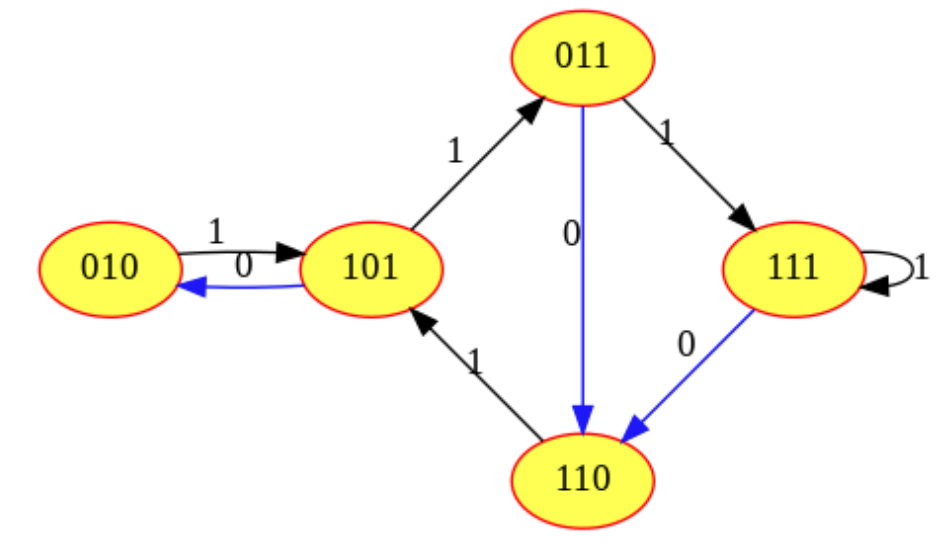
\includegraphics[scale=0.25]{fig/RdB41.png}
    \caption{$(4,1)$-RdB graph.}
    \label{fig:RdB_4_1}
\end{figure}

Denote the $(k,s)$-RdB graph to be $G_{k,s} = (V^{k-1,s},E^{k,s})$, where $V^{k-1,s}$ is the set of all vertices and $E^{k,s}$ is the set of all edges. The following lemmas determining the cardinality of $V^{k-1,s}$ and $E^{k,s}$

\begin{lemma}[\textbf{Number of vertices}]\label{lem:num_V}
    \begin{align}
        \card{ V^{k-1,s}} = \card{ W(k,s)}\label{eq:num_V}
    \end{align}
\end{lemma}
\begin{proof}
    This proof is deduced directly from the construction of $G_{k,s}$ since its set of all vertices is the set of all length $k-1$ sequences containing at most $s$ consecutive letters $0$. 
\end{proof}

\begin{lemma}[\textbf{Number of edges}]\label{lem:num_edges}
    \begin{align}
        \card{ E^{k,s}} = \card{ W(k,s)}\label{eq:card_of_E}
    \end{align}    
\end{lemma}
\begin{proof}
    Observe that for both $\bfx, \bfy\in W(k-1,s)$, if there is an edge from vertex $\bfx = (x_{1},\ldots,x_{k-1})$ to vertex $\bfy = y_{1},\ldots,y_{k-1}$, then $(x_{1},\ldots,x_{k-1},y_{k-1})\in W(k,s)$. 
    
    Besides, for each $s$-RLL sequence $\bfx=(x_{1},\ldots,x_{k})\in W(k,s)$, its prefix and suffix, $(x_{1},\ldots,x_{k-1})$ and $(x_{2},\ldots,x_{k})$, are both $s$-RLL sequence of length $k-1$. Hence, they represent two vertices in the graph $G_{k,s}$ and their connecting edge is represented by the sequence $\bfx$.
    
    So, there is $1-1$ correspondence between $E^{k,s}$ and $W(k,s)$. This results in $\card{ E^{k,s}} = \card{ W(k,s)}$.
\end{proof}

\begin{example}
    According to lemma \ref{lem:num_V} and lemma~\ref{lem:num_edges}, $(4,1)$-RdB graph has $\card{V^{3,1}}=\card{W(3,1)}=5$, and $\card{E^{4,1}} = \card{W(4,1)}=8$. These results can be verified by counting the number of vertices and edges in figure~\ref{fig:RdB_4_1}.
    % Applying lemma \ref{lem:num_V} and lemma~\ref{lem:num_edges} for $k=4,s=1$ gives $\card{V^{3,1}}=\card{W(3,1)}=5$, and $\card{E^{4,1}} = \card{W(4,1)}=8$. Counting the number of edges and vertices in figure~\ref{fig:RdB_4_1} provides the same results
\end{example}

Let $u=(u_{1},u_{2},\ldots,u_{k-1})$ and $v=(v_{1},v_{2},\ldots,v_{k-1})$ be arbitrary vertices in RdB graph. Starting at $v$, the following sequence of edges' labels $(1,u_{1},u_{2},\ldots,u_{k-1})$ apparently forms a proper path going from $v$ to $u$ in RdB graph. Similarly, the sequence of edges' labels $(1,v_{1},v_{2},\ldots,v_{k-1})$ beginning at $u$ is also a directed path from $u$ to $v$. This is sufficient to conclude that the connectivity of RdB graphs is preserved.


% \section{Overview}

% Phần này mô tả tổng quan giải pháp gồm những bước chính nào, hoạt động ra sao. Mục tiêu của phần này là cho người đọc một cái nhìn tổng thể về giải pháp. Để cho dễ hiểu thì nên có một biểu đồ mô tả luồng hoạt động của giải pháp đề xuất. 

% \section{Tên của nội dung chi tiết thứ 1}
% Tên của các chương này đặt theo nội dung mà sinh viên sẽ trình bày trong từng chương. 

% Các chương tiếp theo mô tả chi tiết về các bước, các thuật toán trong giải pháp đề xuất. Có thể trình bày pseudocode cho từng bước. Chú ý, pseudocode chỉ có tác dụng làm chi tiết hoá giải thuật chứ không thay thế được phần thuyết minh về giải thuật. Đối với những chi tiết kỹ thuật khó hiểu nên có các hình minh hoạ để người đọc dễ hiểu. Mỗi một thuật toán/bước thực hiện nên tách ra thành một chương. 

% \section{Tên của nội dung chi tiết thứ 2}



\newpage
%\pagestyle{fancy} % Áp dụng header và footer
\chapter{PROPERTIES OF RUN LENGTH LIMITED DE BRUIJN SEQUENCE}
\label{chapter:pro_rlldb_sequence}
Chapter~\ref{chapter:pro_rlldb_sequence} concerns in determining the rate of \gls{RdB} sequence. Besides, designing efficient encoder and decoder for a longest \gls{RdB} sequence are also critical contributions. 

To calculate the rate and maximal asymptotic rate of \gls{RdB} sequence, first, results on the maximal length of a \gls{RdB} sequence are presented. After that, efficient algorithms to generate a longest RdB sequence and locate any sub-sequence in such sequence are also provided.

\section{Longest simple path in RdB graph}\label{sec:graph_representation}
The rate of de Bruijn sequences can be determined by understanding its longest length. Section \ref{sec:rate} provides a formal definition of rate and maximal asymptotic rate of the de Bruijn sequence. This section concerns finding the longest simple path in $G_{k,s}$, which corresponds to the longest $(k,s)$-RdB sequence.

Let $N(k,s)$ is the maximal length of a $(k,s)$-RdB sequence, and $\ell(G_{k,s})$ be the length of the longest simple path in $G_{k,s}$. Recall that a length $l$ simple path in $G_{k,s}$ is equivalent to a $(k,s)$-RdB sequence of length $l+k-1$. Therefore, $N(k,s) = \ell(G_{k,s})+k-1$. 

The de Bruijn graph $G_{k}$ is actually an Eulerian graph because each vertex has exactly two in-coming edges and two out-coming edges. This results in its longest path visiting each edge exactly once and has a length of $2^{k}$. However, $(k,s)$-RdB graph $G_{k,s}$ doesn't have the same property since the in-degree and out-degree of each vertex can be one or two. Thus, a simple path that visits all edges of the graph may not exist. 

To overcome this issue, the upper bound $\mathbb{U}(k,s)$ for the length of the longest simple path is first determined in this section. Then, $\mathcal{U}(k,s)=\mathbb{U}(k,s)+k-1$ is the upper bound for the length of longest $(k,s)$-RdB sequence. This work later proves that such bound can be achieved by proposing an efficient encoder returning a sequence of length $\mathcal{U}(k,s)$ in section \ref{subsect:encoder}. Hence, it's sufficient to conclude that the upper bound $\mathbb{U}(k,s)$ is also the length of the longest simple path. In other words, $\ell(G_{k,s})=\mathbb{U}(k,s)$, and $N(k,s)=\mathcal{U}(k,s)$

Before deriving the explicit formula of maximal length, it's necessary to analyze more meticulously the in-degree and out-degree of all vertices. Given $0\leq i,j\leq s$, define:

\begin{align*}
    V^{k-1,s}_{i,j} = \Bigl\{ \bfx: \bfx\in V^{k-1,s}, &x[1,i+1]=0^{i}1,  \\
    &x[k-1-j,k-1]=10^{j} \Bigl\}
\end{align*}

That is, $V^{k-1,s}_{i,j}$ is the set of all vertices in $G_{k,s}$ satisfying the first $i+1$ letters are $(0,0,\ldots,0,1)$ and the last $j+1$ letters are $(1,0,0,\ldots,0)$. Lemma~\ref{lem_prop_of_V_ks_ij} summaries the properties of $V^{k-1,s}_{i,j}$ the helps finding $\mathbb{U}(k,s)$.

\begin{lemma}[\textbf{Properties of $V^{k-1,s}_{i,j}$}]\label{lem_prop_of_V_ks_ij}
    {\color{white}.}
    
    % \begin{itemize}
    %     \item $\card{ V^{k-1,s}_{i,j}} = \card{ W(k-i-j-3,s)} $.
    %     \item $\sum_{0\leq i,j\leq s}\card{ V^{k-1,s}_{i,j}} = \card{ V^{k-1,s}}\ (= \card{ W(k-1,s)})$.
    %     \item The in-degree and out-degree of each vertex in $V^{k-1,s}_{i,j}$ (if $V^{k-1,s}_{i,j}\neq\emptyset$) is exactly $1$.
    %     \item The in-degree and out-degree of each vertex in $V^{k-1,s}_{i,j}$ is exactly $1$ for all $0\leq i,j\leq s-1$.
    %     \item For each vertex in $V^{k-1,s}_{s,i}\ (0\leq i\leq s-1)$, their in-degree is exactly one and their out-degree is exactly two.
    %     \item For each vertex in $V^{k-1,s}_{i,s}\ (0\leq i\leq s-1)$, their in-degree is exactly two and their out-degree is exactly one.
    % \end{itemize}
    
    \begin{enumerate}
        \item $\card{ V^{k-1,s}_{i,j}} = \card{ W(k-i-j-3,s)} $.
        \item $\sum_{0\leq i,j\leq s}\card{ V^{k-1,s}_{i,j}} = \card{ V^{k-1,s}}\ (= \card{ W(k-1,s)})$.
        \item The in-degree and out-degree of each vertex in $V^{k-1,s}_{s,S}$ (if $V^{k-1,s}_{s,s}\neq\emptyset$) is exactly $1$.
        \item The in-degree and out-degree of each vertex in $V^{k-1,s}_{i,j}$ is exactly $1$ for all $0\leq i,j\leq s-1$.
        \item For each vertex in $V^{k-1,s}_{s,i}\ (0\leq i\leq s-1)$, their in-degree is exactly one and their out-degree is exactly two.
        \item For each vertex in $V^{k-1,s}_{i,s}\ (0\leq i\leq s-1)$, their in-degree is exactly two and their out-degree is exactly one.
    \end{enumerate}
\end{lemma}
\begin{proof}
    {\color{white}.}
    
    \begin{enumerate}
        \item For each element $x\in V^{k-1,s}_{i,j}$, its subsequence, $x[i+1,k-2-j]$, can be any sequence of length $k-i-j-3$ such that more than $s$ consecutive letter $0$'s is forbidden. Hence $x[i+1,k-2-j]\in W(k-i-j-3,s)$. Reversely, given an arbitrary sequence $y\in W(k-i-j-3,s)$, the string $0^{i}1y10^{j}$ is a sequence in $V^{k-1,s}_{i,j}$. It comes to the conclusion that there is a bijection from $V^{k-1,s}_{i,j}$ to $W(k-i-j-3,s)$. In other word, $\card{ V^{k-1,s}_{i,j}} = \card{ W(k-i-j-3,s)} $.
        
        \item Since $V^{k-1,s}_{i,j}\cup V^{k-1,s}_{i^{\prime},j^{\prime}} = \emptyset$ with $(i,j)\neq(i^{\prime},j^{\prime})$, and $i,j$ cannot exceed $s$, thus, $\sum_{0\leq i,j\leq s}\card{ V^{k-1,s}_{i,j}} = \card{ V^{k-1,s}}$.
        
        \item The properties from $(3)$ to $(6)$ can be deduced directly by considering the prefix and suffix of each element in those sets.
    \end{enumerate}
\end{proof}


% For example, in case $s=1$, all vertices in $V^{k-1,1}_{1,0}$ has one edge coming in and two edges coming out. Hence, the

% All vertices in $V^{k-1,1}_{0,1}$ has two edges coming in and one edges coming out. Furthermore, among two edges coming out of each vertex $v$ in $V^{k-1,s}_{1,0}$, only one of them coming to a vertex $u$ in $V^{k-1,s}_{0,1}$. Similarly, among two edges coming to each vertex $u$ in $V^{k-1,s}_{0,1}$, only one of them coming from a vertex $v$ in $V^{k-1,s}_{1,0}$. Note that, $\card{ V^{k-1,1}_{0,1}} = \card{ V^{k-1,1}_{1,0}} = \card{ W(k-4,1)}$, therefore, there are precisely $\card{ W(k-4,1)}$ edges, each of which go from a vertex in $V^{k-1,1}_{1,0}$ to a vertex in $V^{k-1,1}_{0,1}$. If we remove all these in 

\begin{theorem}[\textbf{Longest simple path}]\label{theo:maximal_length}
    Let $C=\min{(s-1,k-s-2)}$. The length of the longest path in $G_{k,s}$, $\ell(G_{k,s})$, is equal to $\mathbb{U}(k,s)$, where:
    \begin{align}
        \mathbb{U}(k,s) = \card{ W(k,s)} - \left(\sum_{i=0}^{C}\card{ W(k-i-s-3,s)} - s\right)
    \end{align}
\end{theorem}

As mentioned above, proof of theorem \ref{theo:maximal_length} is divided into 2 parts. While the first one claims $\ell(G_{k,s})\leq\mathbb{U}(k,s)$, the second one shows that there exists a sequence can achieve the length of $\mathbb{U}(k,s)+k-1$. This section provides the proof of the first part (lemma~\ref{lem:upperbound}). Proof for the second part is available in section \ref{sec:construction}. 
    
\begin{lemma}\label{lem:upperbound}
    The longest simple path in $G_{k,s}$'s length cannot exceed $\mathbb{U}(k,s)$, that is, $\ell(k,s)\leq\mathbb{U}(k,s)$.
\end{lemma}
    The following definitions and claims are essential to prove lemma~\ref{lem:upperbound}.  
    
\begin{definition}[Balance and unbalanced vertex]
    A vertex with the quantity of in-coming edge equal to the quantity of out-coming edge is called a balanced vertex. A vertex is left-unbalanced if it has $2$ edges coming in and $1$ edges coming out. Reversely, a vertex is right-unbalanced if it has $1$ edge coming in and $2$ edges coming out.
\end{definition}

% {\color{red} Define a path to be a sequence of edges: $e_{1},e_{2},\cdots,e_{n}$ such that $\tau(e_{i})=\sigma(e_{i+1})$ where $\sigma(e_{i})$ and $\tau(e_{i})$ are initial state and terminal state of edge $e_{i}$ respectively}.

Recall that a path is defined to be a sequence of edges. A vertex $v$ is said to be (lying) in or belong to a path $\mathcal{P}$, denoted by $v\in\mathscr{P}$, if $v$ has edges in $\mathcal{P}$. It's also fair to say that $\mathcal{P}$ goes through $v$. Besides, $v$ is called the end (or the start) vertex of $\mathcal{P}$ if its last (first) edge ends (begins) at $v$.

Suppose $\mathscr{P}$ to be a longest simple path in $G_{k,s}$. In other word, $\mathscr{P}$ achieves the length $\ell(G_{k,s})$. Some observations about $\mathscr{P}$ are given in the following claims.
\begin{claim}\label{claim:equal_n_edges}
    All the vertices in $\mathscr{P}$, if not a start or end vertex, must have the number of in-edges and out-edges equal in $\mathscr{P}$.
\end{claim}
\begin{proof}
    Let $v$ be a vertex in $\mathscr{P}$, $v$ is neither start nor end vertex. Then whenever $\mathscr{P}$ comes to $v$ by an in-edge, it must go out of $v$ by an out-edge. So the claim \ref{claim:equal_n_edges} is true.
\end{proof}

% \begin{claim}\label{claim:p_not_cycle}
%     The longest simple path $\mathscr{P}$ is not a cycle.
% \end{claim}
% \begin{proof}
%     Let $\mathscr{P} = (e_{1},e_{2},\ldots,e_{n})$. Denote $\pi(e)$ and $\tau(e)$ to be initial and terminate vertices of $e$ respectively.
    
%     Assume to the contrary that $\mathscr{P}$ is a cycle. Then $\tau(e_{i})=\pi(e_{i+1})$ for all $1\leq i\leq n$, where $e_{n+1}=e_{1}$. 
    
%     \begin{enumerate}
%         \item It can be proved that there is an edge $e^{\prime}\notin \mathscr{P}$ such that either its terminal or its initial vertex $v$ is in $\mathscr{P}$.
%         \begin{itemize}
%             \item If all of vertices in $\mathscr{P}$ are balanced, since RdB graph is connected, there exists an edge (either in or out) of an vertex, for instance, $\tau(e_{i})\in\mathscr{P}$ connecting to an unbalanced vertex $u\notin\mathscr{P}$.
%             \item Otherwise, without loss of generalization, let $\tau(e_{i})$ be an left-unbalanced vertex. Since the number of in-edges and out-edges of $\tau(e_{i})$ equal (by claim~\ref{claim:equal_n_edges}), one out-edge $e^{\prime}$ of $\tau(e_{i})$ doesn't belong to $\mathscr{P}$.
%         \end{itemize}
%         \item Suppose that $e^{\prim}$ is such an edge, and $\pi(e^{\prime})=\tau(e_{i})$. Then the simple path $(e_{i+1},e_{i+2},\ldots,e_{i},e^{\prime})$ is a proper path in RdB, but longer than $\mathscr{P}$, which is a contradiction. 
%     \end{enumerate}
%     The proof is complete.
% \end{proof}

\begin{claim}\label{claim:balance_ver}
    Every balance vertex in $\mathscr{P}$ has their quantity of in-edges and out-edges in $\mathscr{P}$ equal, even if one of them is the start or end vertex.
\end{claim}
\begin{proof}
    Let $v$ be a balanced vertex and $\mathscr{P}$ goes through $v$. If $v$ is neither end nor start vertex, by claim~\ref{claim:balance_ver}, $v$ has the number of in-edges and out-edges in $\mathscr{P}$ equal. 
    
    Without loss of generality, assume that $v$ is the start vertex. This results in the number of out-edges of $v$ being equal or has $1$ edges more than its number of out-edges. If these two quantities are equal, the proof is done. Otherwise, denote $e^{\prime}$ to be one of $v$'s in-edges not belonging to $\mathscr{P}$. Then the path $\mathscr{P}_{1} = \{e^{\prime}\}\cup\mathscr{P}$ beginning at $e^{\prime}$ is a proper simple path RdB graph, but longer than $\mathscr{P}$, which contradicts to the assumption about the longest property of $\mathscr{P}$.
\end{proof}
\begin{claim}\label{claim:shortes_right-left}
    Let $u=0^{s}1x1_{t}0^{j}$ be a right-unbalanced vertex. Then the shortest path going from $u$ to an arbitrary left-unbalanced vertex lengthen $s-j$.
\end{claim}
\begin{proof}
    A left-unbalanced vertex is represented by a sequence whose suffix of length $s$ is filled by $0$. Hence, a path from $u$ to a left-unbalanced vertex must contain at least $s-j$ edges labeled $0$. In fact, a path of length $s-j$ connecting $u$ to a left-unbalanced vertex exists, which is the path of all $0$ labeled edges. This path comes from $u$ to $0^{s-j}1x1_{t}0^{s}$.
\end{proof}
% \begin{proof}
%     Let $v$ be a vertex in $\ell(G_{k,s})$. We just need to consider if $v$ is start or end vertex, the other cases have already been proved by claim \ref{claim:equal_n_edges}.
    
%     Assume that $v$ is the start vertex and suppose to the contrary 
% \end{proof}

\begin{proof}[Proof for lemma~\ref{lem:upperbound}]
    Define $1x1_{t}$ to be a sequence of length $t$ such that start and end letters are both $1$. Let $$\mathscr{L}=\bigcup_{j=0}^{C}\left\{\bfu:\bfu=0^{j}1x1_{t}0^{s},s+t+j=k-1\right\}$$ be the set of all left-unbalanced vertices
    
    Let $\bfv=0^{j}1x1_{t}0^{s}$ be an arbitrary vertex in $\mathscr{L}$ such that $\bfv$ isn't the end-vertex of path $\mathscr{P}$. 
    
    \begin{enumerate}
        \item It can be proved that there is a path $\mathcal{P}_{v}$ of length $s-j$ satisfying all of its edges not lying in $\mathscr{P}$ and its end-vertex is $\bfv$.
            The path $\mathcal{P}_{v}$ is constructed backwardly as follows:
            
            Starts with $\mathcal{P}_{v}=\emptyset$. As $\bfv$ has $2$ in-edges and $1$ out-edges, there's at least $1$ in-edge $e_{v}$ of $\bfv$ not lying in $\mathscr{P}$. Of course, $e_{v}$'s label is $0$. Adds $e_{v}$ to $\mathscr{P}_{v}$. Let $a_{1}0^{j}1x1_{t}0^{s-1}= \pi(e_{v})$ be the initial state of $e_{v}$. If $\pi(e_{v})$ is a balance vertex, then by the claim \ref{claim:balance_ver}, there also must be at least $1$ in-edge of $\pi(e_{v})$ not lying in $\mathscr{P}$. Continue adding this edge to the head of $\mathcal{P}_{v}$. Denote $a_{2}a_{1}0^{j}1x10^{s-2}$ to be the initial state of this edge. Now, $\mathcal{P}_{v}$ can be represented as below:
            
            \[\mathcal{P}_{v}=\left[\left(a_{2}a_{1}0^{j}1x1_{t}0^{s-2},a_{1}0^{j}1x1_{t}0^{s-1}\right), \left(a_{1}0^{j}1x1_{t}0^{s-1},0^{j}1x1_{t}0^{s}\right)\right]\]
            
            Assume inductively that:
            
            \begin{align*}
                \mathcal{P}_{v}= \Bigl[&\left(a_{l}\cdots a_{2}a_{1}0^{j}1x1_{t}0^{s-l},a_{l-1}\cdots a_{1}0^{j}1x1_{t}0^{s-(l-1)}\right),\cdots,\\
                &\left(a_{2}a_{1}0^{j}1x1_{t}0^{s-2}, a_{1}0^{j-1}1x1_{t}0^{s-1}\right),\\
                &\left(a_{1}0^{j-1}1x1_{t}0^{s-1},0^{j}1x1_{t}0^{s}\right)\Bigl]   
            \end{align*}
            with $l\leq s-j$.
            
            If $l=s-j$, the proof is done. Otherwise, it's obvious that $$a_{l}\cdots a_{2}a_{1}0^{j}1x1_{t}0^{s-l}$$ is balance, hence, by claim \ref{claim:balance_ver}, it also has at least $1$ in-edge not lying in $\mathscr{P}$, and one can continue adding such edge to the head of $\mathcal{P}_{v}$.
            
        \item It can be shown that for each $u,v\in\mathscr{L}$ such that neither $u$ nor $v$ is the end vertex of the last edge of $\mathscr{P}$, paths $\mathcal{P}_{u}$ and $\mathcal{P}_{v}$ are edge-disjoint.
    
            Represent $\mathcal{P}_{u} = [e_{u,1},e_{u,2},\cdots,e_{u,i}]$, $\mathcal{P}_{v}=[e_{v,1},e_{v,2},\cdots,e_{v,j}]$. Assume to the contrary that $\exists t\leq i,l\leq j$ satisfying $e_{u,t}=e_{v,l}$. Without loss of generalization, we suppose that $i-t\leq j-l$. As all edges in $\mathcal{P}_{u}$ and $\mathcal{P}_{v}$ are labeled $0$, we must have $e_{u,t+1}=e_{v,l+1},\cdots,e_{u,i}=e_{v,l+(i-t)}$. 
            
            If $l+i-t=j$, we have $\mathcal{P}_{u}$ and $\mathcal{P}_{v}$ have the same last edge but different terminal states, which is impossible. Otherwise, the path $e_{v,l+i-t+1},\cdots,e_{v,j}$ is the path connecting $u$ to $v$. But the length of this path is smaller than $s$, which is also absurd.
    \end{enumerate}
    % $(1)$ It can be proved that there is a path $\mathcal{P}_{v}$ of length $s-j$ satisfying all of its edges not lying in $\mathscr{P}$ and its end-vertex is $\bfv$.
    
    % The path $\mathcal{P}_{v}$ is constructed backwardly as follow:
    
    % Starts with $\mathcal{P}_{v}=\emptyset$. As $\bfv$ has $2$ in-edges and $1$ out-edges, there's at least $1$ in-edge $e_{v}$ of $\bfv$ not lying in $\mathscr{P}$. Of course, $e_{v}$'s label is $0$. Adds $e_{v}$ to $\mathscr{P}_{v}$. Let $a_{1}0^{j}1x1_{t}0^{s-1}= \pi(e_{v})$ be the initial state of $e_{v}$. If $\pi(e_{v})$ is a balance vertex, then by the claim \ref{claim:balance_ver}, there also must be at least $1$ in-edge of $\pi(e_{v})$ not lying in $\mathscr{P}$. Continue adding this edge to the head of $\mathcal{P}_{v}$. Denote $a_{2}a_{1}0^{j}1x10^{s-2}$ to be the initial state of this edge. Now, $\mathcal{P}_{v}$ can be represented as below:
    
    % $\mathcal{P}_{v}=[\left(a_{2}a_{1}0^{j}1x1_{t}0^{s-2},a_{1}0^{j}1x1_{t}0^{s-1}\right), \left(a_{1}0^{j}1x1_{t}0^{s-1},0^{j}1x1_{t}0^{s}\right)]$
    
    % Assume inductively that:
    
    % \begin{align*}
    %     \mathcal{P}_{v}= \Bigl[&\left(a_{l}\cdots a_{2}a_{1}0^{j}1x1_{t}0^{s-l},a_{l-1}\cdots a_{1}0^{j}1x1_{t}0^{s-(l-1)}\right),\cdots,\\
    %     &\left(a_{2}a_{1}0^{j}1x1_{t}0^{s-2}, a_{1}0^{j-1}1x1_{t}0^{s-1}\right),\\
    %     &\left(a_{1}0^{j-1}1x1_{t}0^{s-1},0^{j}1x1_{t}0^{s}\right)\Bigl]   
    % \end{align*}
    % with $l\leq s-j$.
    
    % If $l=s-j$, the proof is done. Otherwise, it's obvious that $a_{l}\cdots a_{2}a_{1}0^{j}1x1_{t}0^{s-l}$ is balance, hence, by claim \ref{claim:balance_ver}, it also has at least $1$ in-edge not lying in $\mathscr{P}$, and one can continue adding such edge to the head of $\mathcal{P}_{v}$.
    
    % $(2)$ It can be shown that for each $u,v\in\mathscr{L}$ such that neither $u$ nor $v$ is the end vertex of the last edge of $\mathscr{P}$, paths $\mathcal{P}_{u}$ and $\mathcal{P}_{v}$ are edge-disjoint.
    
    % Represent $\mathcal{P}_{u} = [e_{u,1},e_{u,2},\cdots,e_{u,i}]$, $\mathcal{P}_{v}=[e_{v,1},e_{v,2},\cdots,e_{v,j}]$. Assume to the contrary that $\exists t\leq i,l\leq j$ satisfying $e_{u,t}=e_{v,l}$. Without loss of generalization, we suppose that $i-t\leq j-l$. As all edges in $\mathcal{P}_{u}$ and $\mathcal{P}_{v}$ are labeled $0$, we must have $e_{u,t+1}=e_{v,l+1},\cdots,e_{u,i}=e_{v,l+(i-t)}$. 
    
    % If $l+i-t=j$, we have $\mathcal{P}_{u}$ and $\mathcal{P}_{v}$ have the same last edge but different terminal states, which is impossible. Otherwise, the path $e_{v,l+i-t+1},\cdots,e_{v,j}$ is the path connecting $u$ to $v$. But the length of this path is smaller than $s$, which is also absurd.
    
    Summary, for each vertex in $\mathscr{L}$ such that $v$ isn't the end-vertex of the last edge in path $\mathscr{P}$, there is a path $\mathcal{P}_{v}$ of length $s-j$ satisfying all of its edges not lying in $\mathscr{P}$ and takes $v$ to be its end-vertex. Moreover, all these such paths are edge-disjoint, and there can be only $1$ end-vertex of the last edge in path $\ell(G_{k,s})$, the total edges of all such path $\mathcal{P}_{u}$ is:
    \begin{align*}
        \sum_{i=0,i\neq j}^{C} &(s-i)\lvert W(k-s-i-3,s) \rvert \\
        + &(s-j)(\lvert W(k-s-j-3,s)\rvert-1)\\
        = \sum_{i=0}^{C} &(s-i)\lvert W(k-s-i-3,s) \rvert - (s-j) \\
        \geq \sum_{i=0}^{C} &(s-i)\lvert W(k-s-i-3,s) \rvert -s  
    \end{align*}
    This means at least $\sum_{i=0}^{C} (s-i)\lvert W(k-s-i-3,s) \rvert -s$ edges not lying in $\mathscr{P}$. As the number of edges in $(k,s)$-RdB is $\lvert W(k,s)\rvert$, the length of the longest path $\mathscr{P}$ can not exceed : 
    \[\lvert W(k,s)\rvert - (\sum_{i=0}^{C} (s-i)\lvert W(k-s-i-3,s) \rvert- s)\]
    This concludes our lemma.
\end{proof}

Define $\mathcal{U}(k,s) = \mathbb{U}(k,s)+(k-1)$, then $\mathcal{U}(k,s)$ is length of the longest $(k,s)$-RdB sequence.

\section{Rate and maximal asymptotic rate of \texorpdfstring{$(k,s)$}{(k,s)}-RdB sequence}\label{sec:rate}
For every $(k,s)$-RdB sequence, their rate is defined as follows:
\begin{definition}[Rate]
    Denote $R(\bfx_{k,s})$ to be the rate of a $(k,s)$-RdB sequence $\bfx_{k,s}$, then:
    \begin{align}
        R(\bfx_{k,s}) = \dfrac{\log\left(\card{\bfx_{k,s}}\right)}{k}
    \end{align}
    where the base of logarithm function is $\left\lvert\Sigma\right\rvert=2$.
\end{definition}

The rates of sequences are the proportion of the data-stream that is useful (non-redundant), tell how much useful information is transmitted. The sequence's rate actually originates from information rate. Recall that, in definition~\ref{def:information_rate}, the rate $R_{C}$ of a code $C$ consisting of length $n$ $q$-ary sequences is $R_{C}=\dfrac{\log_{q}\left(\card{C}\right)}{n}$. If a $(k,s)$-RdB sequence $x_{k,s}$ is considered to be a code $C_{k,s}$, each of its size $k$ windows is treated as a codeword. The size of $C_{k,s}$ is exactly the length of $x_{k,s}$ minus $k$, but the offset $k$ can be omitted under log calculation. Hence: $$R_{C_{k,s}}= \dfrac{\log_{q}\left(\card{C_{k,s}}\right)}{n} = \dfrac{\log(\card{\bfx_{k,s}})}{k} = R(x_{k,s})$$. That is to say, $R(\bfx_{k,s})$ is eventually a kind of information rate.

Note that, a high rate is usually preferred. Accordingly, with each given pair $(k,s)$, the maximal rate of all $(k,s)$-RdB sequence is defined.
\begin{definition}[Maximal rate]
    Given $k$ and $s$, the maximal rate $R_{k,s}$ of all $(k,s)$-RdB sequences is:
    \begin{align}
        R_{k,s} = \dfrac{\log(N(k,s))}{k}
    \end{align}
\end{definition}

% For the rate $R_{k,s}$, if one cares about the very large $k$, it is when the maximal asymptotic rate of sequence comes to play.

The maximal asymptotic rate is concerned in case $k$ appears to be very large.
\begin{definition}[Maximal asymptotic rate]
    Denote $R_{s}$ to be the maximal asymptotic rate of $(k,s)$-RdB sequences, then:
    \begin{align}
        R_{s} = \lim_{k\to\infty}\dfrac{\log(N(k,s))}{k}
    \end{align}
\end{definition}

Having the explicit formula of $N(k,s)$ determined makes it easier to calculate the maximal asymptotic rate of the $(k,s)$-RdB sequence. The following equation is a direct consequence of theorem~\ref{theo:maximal_length}:
\begin{align}
    N(k,s) = \card{ W(k,s)} - \left(\sum_{i=0}^{C}\card{ W(k-i-s-3,s)} - s\right) + k - 1\label{eq:N_k_s}
\end{align}


Theorem \ref{theo:rate_1} below shows that the rate of $(k,1)$-RdB sequence is better than the rate of Hybrid de Bruijn sequence. Therefore, it's able to use $(k,1)$-RdB sequence for the system in \cite{zhang2021timing} instead to increase rate, speed of encoding and decoding for the transmitted signals.

\begin{theorem}\label{theo:rate_1}
    \begin{align}
        R_{1} = 0.6942
    \end{align}
\end{theorem}
\begin{proof}
    Substitute $s=1$ into expression~\ref{eq:N_k_s} gives $N(k,1) = \card{W(k,1)} - \card{W(k-4,1)}$, and recall that $\{\card{W(k,1)}\}$ is a Fibonacci sequence with: 
    \[\card{W(k,1)} = \dfrac{\phi^{k+2}+\varphi^{k+2}}{\sqrt{5}}\].
    where $\phi = \dfrac{1+\sqrt{5}}{2}$ and $\varphi = \dfrac{1-\sqrt{5}}{2}$. Here, observe that $\phi\varphi=-1$, so $\phi^{2}\varphi^{2}=1$, consequently, it's able to write:
    \begin{align*}
        \left\{\begin{matrix}
            \phi^{-2} = \varphi^{2} \\
            \varphi^{-2} = \phi^{2}
        \end{matrix}\right.
    \end{align*}
    As a result: 
    \begin{align*}
        \card{W(k,1)} - \card{W(k-4,1)} &= \dfrac{\phi^{k+2}+\varphi^{k+2}}{\sqrt{5}} - \dfrac{\phi^{k-2}+\varphi^{k-2}}{\sqrt{5}}\\
        &= \dfrac{\phi^{k+2}+\varphi^{k+2}-\phi^{k}\varphi^{2}-\varphi^{k}\phi^{2}}{\sqrt{5}}\\
        &= \left(\phi^{k}+\varphi^{k}\right).\dfrac{\phi^{2}-\varphi^{2}}{\sqrt{5}}
    \end{align*}
    And hence:
    \begin{align*}
        R_{1} &= \lim_{k\to\infty}\dfrac{\log(N(k,1))}{k} \\
        &= \lim_{k\to\infty}\dfrac{ \log\left( \left(\phi^{k}+\varphi^{k}\right).\dfrac{\phi^{2}-\varphi^{2}}{\sqrt{5}}+k \right) }{k} \\
        &= \log(\phi) \approx 0.6942
    \end{align*}
\end{proof}

The following theorem is the generalization of theorem \ref{theo:rate_1}.
\begin{theorem}[Maximal asymptotic rate of RdB sequence]\label{theo:rate_s}
    Let $k$ be a positive integer. Then:
    \begin{align}
        R_{s} = \log(\lvert\omega\rvert)
    \end{align}
    where $\omega$ is the root of equation: %\inlineequation[eq:inline]{x^{s+1}-x^{s}-\ldots-x-1 = 0}
    \begin{equation}
        x^{s+1}-x^{s}-\ldots-x-1 = 0\label{eq:char_eq}
    \end{equation}
    such that $\lvert\omega\rvert$ is largest.
\end{theorem}
\begin{proof}
    
    The root $\omega$ is actually a Pisot number. More particularly, $\omega$ is the only positive roots of~\ref{eq:char_eq} lying in the interval $(1,2)$, the other roots are in the open disk $\left\{z\in\mathbb{C},\card{z}<1\right\}$. Also, note that $x^{s+1}-x^{s}-\ldots-x-1=0$ is the characteristic equation of $W(k,s)$. Therefore, with $k$ big enough, $\card{W(k,s)}$ can be estimated as follows: \[\card{W(k,s)} \approx a.\lvert\omega\rvert^{k}\] whereas $a$ is a positive constant. Thus, from expression~\ref{eq:N_k_s}:
    \begin{align*}
        N(k,s) &= \card{ W(k,s)} - \left(\sum_{i=0}^{C}\card{ W(k-i-s-3,s)} - s\right) + k - 1 \\
        &\approx \sum_{t=k-s}^{k}(k-t+1)a\lvert\omega\rvert^{t-2} + s + k - 1\\
        &= \lvert\omega\rvert^{k-s-2}\left( \sum_{t=k-s}^{k}a(k-t+1)\lvert\omega\rvert^{t-k+s} + \dfrac{s+k-1}{\lvert\omega\rvert^{k-s-2}}\right)\\
        &= \lvert\omega\rvert^{k-s-2}\left( \sum_{i=0}^{s}a(i+1)\lvert\omega\rvert^{s-1} + \dfrac{s+k-1}{\lvert\omega\rvert^{k-s-2}}\right) 
    \end{align*}

    This results in:
    \begin{align*}
        R_{k} &= \lim_{k\to\infty}\dfrac{\log\left( \lvert\omega\rvert^{k-s-2}\left(\sum_{i=0}^{s}a(i+1)\lvert\omega\rvert^{s-1}+\dfrac{s+k-1}{\lvert\omega\rvert^{k-s-2}}\right)\right)}{k} \\
        &= \lim_{k\to\infty}\dfrac{(k-s-2)\log(\lvert\omega\rvert)}{k} + \lim_{k\to\infty}\dfrac{\log\left(\sum_{i=0}^{s}a(i+1)\lvert\omega\rvert^{s-i}+\dfrac{s+k-1}{\lvert\omega\rvert^{k-s-2}}\right)}{k}\\
        &= \log(\lvert\omega\rvert)
    \end{align*}
    
\end{proof}
% \begin{figure*}[!ht]
%     \centering
%       \begin{subfigure}{0.9\linewidth}
%         \centering
%         \includegraphics[scale=0.23]{fig/Legend.png}
%         \label{fig:neg_size}
%         \end{subfigure}
%         %\quad
%       \begin{subfigure}{0.4\linewidth}
%         \centering
%         \includegraphics[scale=0.35]{fig/train_percent_Hit@1.pdf}
%         \caption{Hit@1}
%         \label{fig:sub_hit1}
%         \end{subfigure}
%         %\quad
%       \begin{subfigure}{0.4\linewidth}
%         \centering
%         \includegraphics[scale=0.35]{fig/train_percent_Hit@10.pdf}
%         \caption{Hit@10}
%         \label{fig:sub_hit10}
%         \end{subfigure}
%         %\quad
%     \begin{subfigure}{0.4\linewidth}
%         \centering
%         \includegraphics[scale=0.35]{fig/train_percent_MRR.pdf}
%         \caption{MRR}
%         \label{fig:sub_mrr}
%         \end{subfigure}
%     \caption{Saving of labelling effort for entity alignment on D-W-V1 test set}
%     \label{fig:supervision_percent}
%  \end{figure*}

\section{Construction of RdB sequence}\label{sec:construction}
% {\color{red} Need paraphrase to avoid self-plagiarism\color{blue}

This section presents a construction of a $(k,s)$-RdB sequence $\bfc_{k,s}$. Furthermore, given a substring of length $k$ of the sequence $\bfc_{k,s}$, a fast decoding algorithm to determine the location of the given substring is provided. The complexity of the decoding algorithm is sub-linear with respect to the length of $\bfc_{k,s}$. There are some classical de Bruijn sequences with sub-linear decoding algorithm \cite{mitchell1996method,tuliani2001bruijn,kociumaka2016efficient}. This work uses the minimal de Bruijn sequence, constructed in \cite{kociumaka2016efficient,fredricksen1978necklaces}, and some special properties of Lyndon words to construct a $(k,s)$-RdB.
% }

\begin{definition}[\textbf{Lyndon words}]
    A sequence $w$ is a Lyndon word if and only if it's strictly smaller than all of its rotation.
\end{definition}
For more intelligible, several Lyndon words and non-Lyndon words are provided in example~\ref{exp:Lyndon}.
\begin{example}[Lyndon words]\label{exp:Lyndon}
    The word $00101$ is a Lyndon word, since it is smaller than all of its rotation: $01010$, $10100$, $01001$, $10010$. The word $01100$ is not a Lyndon word, since one of its rotations, $00011$, is smaller than it. The word $011011$ is also not a Lyndon word, as its cyclic rotation by $3$ letters is equal to it. 
\end{example}

\subsection{Encoder for a\texorpdfstring{$(k,s)$}{(k,s)}-RdB sequence} \label{subsect:encoder}
In 1978, Fredricksen and Maiorana~\cite{fredricksen1978necklaces} proposed the \gls{fkm} algorithm to efficiently construct the lexicographically minimal de Bruijn sequence, which is later called granddaddy sequence by Knuth~\cite{knuth2013art}. The algorithm was based on their finding of the connection between de Bruijn sequence and Lyndon words.

\begin{lemma}[\cite{fredricksen1978necklaces}]\label{lem:FKM}
    The lexicographically minimal de Bruijn sequence of order $k$ ($k$-MdB) is the concatenation of all Lyndon words whose length is a divisor of $k$ in the lexicographically order.
\end{lemma}

For example, the $6$-MdB sequence is decomposed into Lyndon words as follows:
\begin{example}[Decomposition of $6$-MdB sequence]
    Recall that $6$-MdB sequence is already given in example~\ref{exp:granddaddy}, which is:
    \[0000001000011000101000111001001011001101001111010101110110111111\]
    As stated in lemma~\ref{lem:FKM}, it can be decomposed in lexicographically order into Lyndon words listed follows:
    \begin{align*}
        &0\\
        &000001\\
        &000011\\
        &000101\\
        &000111\\
        &001\\
        &001011\\
        &001101\\
        &001111\\
        &01\\
        &010111\\
        &011\\
        &011111\\
        &1
    \end{align*}
\end{example}


This thesis observes that it is able to append a prefix to a suffix of $k$-MdB to obtain a $(k,s)$-RdB sequence, i.e., in the cycle representing $k$-MdB, there are arcs representing $(k,s)$-RdB sequences. To illustrate this idea, figure~\ref{fig:substring_of_circle} gives an example for $k=6$ and $s=2$, where the blue arc and the red arc indicate the prefix and the suffix respectively. Any substring of the concatenation of the prefix and suffix is a $(6,2)$-RdB sequence.

\begin{figure}[htbp]
    \centering
    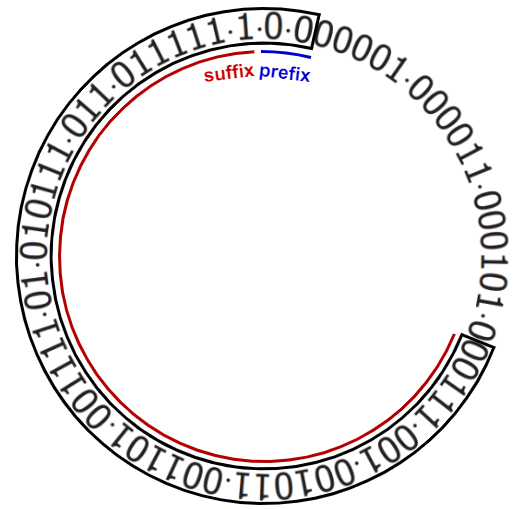
\includegraphics[scale=0.5]{fig/construction/subtring of cyclic.png}
    \caption{Example for $k=6,\ s=2$. In the circle of $6$-MdB, an arbitrary substring of the concatenation of suffix and prefix in the picture is a $(6,2)$-RdB sequence.}
    \label{fig:substring_of_circle}
\end{figure}

% \begin{figure}
%     \centering
%     \input{fig/construction/construction}
%     \caption{Caption}
%     \label{fig:my_label}
% \end{figure}

More precisely, the construction is described as follow:
\begin{construction}\label{constr:encoder}
    Let $\bfx=(x_{1},\ldots,x_{n})$ be the $k$-MdB constructed from Lemma~\ref{lem:FKM} and $u_{k,s}= 0^{s+1}1^{k-s-1}$ be a Lyndon word of length $k$ satisfying the first $s+1$ letters are all $0$'s and the last $k-s-1$ letters are all $1$'s. By the intrinsic property of de Bruijn sequences, there exists only one index $i$ such that $\bfu_{k,s}=\bfx[i,i+k-1]=(x_{i},\ldots,x_{i+k-1})$. Denote the word $\bfc_{k,s} = (x_{i+1},\ldots,x_{n},0,0,\ldots,0)$, obtained by adding $s$ letters $0$ to the end of the suffix of $\bfx$, from index $i+1$ to the end. Theorem \ref{theo:validity} below claims that $\bfc_{k,s}$ is a $(k,s)$-RdB sequence. 
\end{construction}

This thesis later proves that $\bfc_{k,s}$ is even the longest $(k,s)$-RdB sequence. 

Denote \L$_{n}$ to be the set of all Lyndon words of length $n$, and $\text{\L}^{(n)}=\cup_{d\card n}\text{\L}_{d}$ to be the set of all Lyndon words whose lengths are divisors of n. The formal encoder to construct a $(k,s)$-RdB sequence is given in algorithm~\ref{alg:encoder}.

\begin{algorithm}
\DontPrintSemicolon
    \SetKwInOut{KwIn}{Input}
    \SetKwInOut{KwOut}{Output}
    \KwIn{$k$, and descending ordered set \L$^{(n)}$. }
    \KwOut{ $(k,s)$-RLL dBs}
    \BlankLine
        % Find the set of Lyndon words  $S=\left\{\lambda_{i}:\ \lambda_{i}\in\mathsf{L}^{(k)}\right\}$
    
    $\mathbf{w}\gets$emptystring\;
    \For{$\lambda \in$\L$^{(n)}$}{
        $\mathbf{w}.prepend(\lambda)$\;
        \If{$\lambda== 0^{s+1}1^{k-s-1}$}{
            \tcc{remove the first letter of $w$, which is 0, and add $s$ letters $0$ to the end}
            $\mathbf{w} = \mathbf{w}[2,\ell]0^{s}$\;
            \textbf{break}\;
        }
    }
    \KwRet{$\mathbf{w}$}
    \caption{Encode (k,s)-RLL dBs}
    \label{alg:encoder}
\end{algorithm}

The set $\text{\L}^{(n)}$ in lexicographically order can be generated in constant amortized time by applying \gls{fkm} algorithm (analyzed in~\cite{ruskey1992generating}), or by another algorithm developed by Duval in~\cite{duval1988generation}. In algorithm~\ref{alg:encoder}, the most consuming time step is to produce the set $\text{\L}^{(n)}$, and hence, its complexity is the complexity of the algorithm used to bring out $\text{\L}^{(n)}$.
% {\color{red} Runtime of Encoder, critical runtime is at FKM ...}

Here presents an example for $k=6$ and $s=2$. 
\begin{example}[Construction of $(6,2)$-RdB sequence]
    The suffix: $$00111\ 001011\ 001101\ 001111\ 01\ 010111\ 011\ 011111\ 1$$ is taken from the granddaddy of order $6$ given above. Adding $2$ letter $0$ to the end of it obtains:
    \[
        00111\ 00\ 001011\ 001101\ 001111\ 01\ 010111\ 011\ 011111\ 1\ 00
    \]
    which is indeed a $(6,2)$-RdB sequence.
\end{example}
Now, theorem \ref{theo:validity} proves that the Construction~\ref{constr:encoder} always return a $(k,s)$-RdB sequence.

\begin{theorem}\label{theo:validity}
    The sequence $\bfc_{k,s}$ obtained from Construction~\ref{constr:encoder} is a $(k,s)$-RdB sequence.
\end{theorem}
\begin{proof}
    First, it's necessary to show that each substring of length $k$ appears at most once in $\bfc_{k,s}$. Note that the granddaddy sequence $\bfx$ obtained from Lemma~\ref{lem:FKM} is a cyclic de Bruijn sequence, and $\bfc_{k,s}$ is actually a substring of $\bfx$. Hence, $\bfc_{k,s}$ just contains each substring of size $k$ at most once.
    
    Now, claiming that $\bfc_{k,s}$ doesn't contain any patterns $0^{s+1}$ will complete the theorem. This can be proved by considering the property of Lyndon words. It's obvious to see that $\bfu_{k,s}=0^{s+1}1^{k-s-1}$ is the largest Lyndon word containing $s+1$ consecutive symbols $0$. Hence, every Lyndon words decomposed from $\bfc_{k,s}$ doesn't take $0^{s+1}$ as a substring. Moreover, the last symbol of all Lyndon words but $0$ is $1$. Therefore, $0^{s+1}$ will not appear in the combination of Lyndon words larger than $\bfu_{k,s}$. Adding $0^{s}1^{k-s-1}$ to the beginning and $s$ letters $0$ to the end of this combination resulting in $\bfc_{k,s}$ won't change this property. So, it's able to conclude that $\bfc_{k,s}$ is indeed a $(k,s)$-RdB sequence.
\end{proof}

\subsection{Decoder for a \texorpdfstring{$(k,s)$}{(k,s)}-RdB sequence}
In~\cite{zhang2021timing}, the Hybrid de Bruijn sequence of order $k$ after being received needs to be decoded for correcting errors. More particularly, it's necessary to indicating the exact location of an arbitrary sequence of length $k$ in the Hybrid de Bruijn sequence. To do that, they proposed to use look-up table, which is {\color{blue} is an exponential complex method}.

Similarly, it's essential for this work to decode $\bfc_{k,s}$. In 2016, Kociumaka, Radoszewski, and Rytter presented the first sub-linear decoding algorithm $\cD_{KRR}$ for the minimal de Bruijn sequences. And since $\bfc_{k,s}$ is a substring of a minimal de Bruijn sequence, it's able to modify $\cD_{KRR}$ to decode $\bfc_{k,s}$ in sub-linear time. 

Let $i=\cD_{KRR}(\bfu_{k,s})$ be the position of the word $\bfu_{k,s}$ in the granddaddy sequence of order $k$ $\bfx$. Recall that, from Construction~\ref{constr:encoder}, we have $\bfc_{k,s}=(x_{i+1},\ldots,x_{n},0^{s})$. Thus, for each length $k$ word $v$ lying in $\bfc_{k,s}$, its location in $\bfc_{k,s}$ is to location of $v$ in $x$ minus $j$, unless they are of the form $1^{j}0^{k-j}$ for all $1\leq j\leq s$ which appear at the end of $\bfc_{k,s}$. The formal description of our decoding algorithm is shown in algorithm \ref{alg:decode}.

\begin{algorithm}
\DontPrintSemicolon
    \SetKwInOut{KwIn}{Input}
    \SetKwInOut{KwOut}{Output}
    \KwIn{A word $\bfv=(v_1,\ldots,v_k)$ of length $k$}
    \KwOut{a is the location of $\bfv$ in $\bf\bfc_{k,s}$}
    \BlankLine
    
    $i \gets \cD_{KRR}(\bfu_{k,s})$; \\
     \tcc{ $\cD_{KRR}$ is the decoder of the minimal de Bruijn sequence in \cite{kociumaka2016efficient}}
     \If {$\bfv = 1^{j}0^{k-j}$,}{\KwRet{$n-i+1-(k-j)$};}
     \Else{\KwRet{$\cD_{KRR}(\bfv)-i$};}
    \caption{Decode (k,s)-RLL dBs $\bf\bfc_{k,s}$}
    \label{alg:decode}
\end{algorithm}

\subsection{The optimality of our construction}
This section gives proof for the claim stated in section \ref{sec:graph_representation}, that is, the encoder produces sequence $\bfc_{k,s}$ whose length equals to to upper bound $\mathcal{U}(k,s)$, and thus, $\bfc_{k,s}$ is the longest the $(k,s)$-RdB sequence. In order to do so, $\bfc_{k,s}$'s length, denoted by $\ell(\bfc_{k,s})$, is needed calculating first. It's then essential to show that $\ell(\bfc_{k,s})$ is equal to $\mathcal{U}(k,s)$ by some algebraic transformations.

Given a word $u$, denote $\langle u\rangle$ to be its minimal rotation. For instance, the minimal rotation of 010110 is 001011, or, the minimal rotation of 010101 is itself. For every word $v$, we define:
\begin{align*}
    S(v) = \left\{u: u\in\Sigma^{\card{ v}},\langle u\rangle\leq v\right\}
\end{align*}
to be the set of all sequence of length $\card{ v}$ satisfying their minimal rotation don't exceed $v$. The following example~\ref{exp:S_v} lists all element of $S(v)$ with $v=01101$.
\begin{example}[Example of $S(v)$]\label{exp:S_v}
    Given $v= 01101$, all sequence of length $\card{v}=5$ whose minimal rotations are at most $v$ is:
    \begin{align*}
        S(01101) = \bigl\{ &00000,\\
        &00001,00010,00100,01000,10000, \\
        &00011,00110,01100,11000,10001, \\
        &00111,01110,11100,11001,10011 \bigl\}
    \end{align*}
\end{example}
If $v$ is a Lyndon word, Lemma 29 in \cite{kociumaka2016efficient} tells that the cardinality of $S(v)$, $\card{ S(v)}$, equals to the length of the prefix of the granddaddy sequence $x$, from the beginning to the sub-string $v$. Recall that $\bfu_{k,s}$ is also a Lyndon word, one have:
\begin{align}
    \card{ S(\bfu_{k,s})} &= 2^{k}- (\ell(\bfc_{k,s}) - (k-1) -s ) \nonumber\\
    \Leftrightarrow  \ell(\bfc_{k,s}) &= 2^{k}+(k-1)+s-\card{ S(\bfu_{k,s})} \label{eq:cks&sks}
\end{align}

This brings the idea determining $\ell(\bfc_{k,s})$ by computing the size of the set $S(\bfu_{k,s})$. 
\begin{lemma}\label{lem:card_S_uks}
    Let $A_{t} = 2^{t-2}$ for all $t>1$, $A_{1}=1$, and $M=\max{(k-s,s+3)}$. Then:
    \begin{align}
        \card{ S(\bfu_{k,s})}= 1 + \sum_{t=M}^{k}(k-t+1)\card{C(t-2,s)} + \sum_{t=1}^{k-s-1}A_{t} \label{eq:card_S_uks}
    \end{align}
\end{lemma}
\begin{proof}
    Let $i,j$ be two non-negative integers such that $i+j<k$, denote:
    $$U_{i,j}= \left\{0^{i}1x1_{t}0^{j}\in S(\bfu_{k,s}): i+j+t=k\right\}$$
    to be the set of all words in $S(\bfu_{k,s})$ satisfying its prefix of length $i+1$ is $0^{i}1$ and its suffix of length $j+1$ is $10^{j}$.
    
    Since $S(\bfu_{k,s})$ is the disjoint union of $0^k$ and all sets $U_{i,j}$ for $i,j \geq 0$ and $i+j<k$, we obtain:
    \begin{equation}\label{eq:s=1+2u}
        \card{S(\bfu_{k,s})}= 1 +\sum_{\substack{i,j\geq 0 ; i+j \leq s}} \card{U_{i,j}}+\sum_{\substack{i,j\geq 0 ; s < i+j<k}} \card{U_{i,j}}.
    \end{equation}
    
    If we fix $1\leq t \leq k$, there are $k-t+1$ pairs $(i,j)$ such that $t=k-i-j$. If $i+j \leq s$ then the sub-string $1x1_{t}$ must contain $s+1$ consecutive 0's (consequently, $k-i-1-(i+2)+1\geq s+1\Rightarrow t=k-i-j\geq s+3$), and therefore, $\card{U_{i,j}}=\card{C(t-2,s)}.$ 
    Hence,
    \begin{equation}\label{eq:c1}
        \cC_1= \sum_{\substack{i,j\geq 0 ;\\ i+j \leq s}} \card{U_{i,j}} = \sum_{t=M}^{k}(k-t+1)\card{C(t-2,s)}. 
    \end{equation}
    where $M=\max(s+3,k-s)$.
    
    If $k>i+j > s$ then the sub-string $(x_{i+2},\ldots,x_{k-j-1})$ can be any word of length $t-2$ and thus $\card{U_{i,j}}=A_t=2^{t-2}$. Hence:
    \begin{equation}\label{eq:c2}
        \cC_2=\sum_{\substack{i,j\geq 0 ;\\ s< i+j<k}} \card{U_{i,j}}= \sum_{t=1}^{k-s-1}(k-t+1)A_{t}.
    \end{equation}
    From Equations (\ref{eq:s=1+2u}), (\ref{eq:c1}), (\ref{eq:c2}), we get the result in Lemma \ref{lem:card_S_uks}.
\end{proof}

Combining the results from Lemma~\ref{lem:card_S_uks} and equation~\ref{eq:cks&sks} gives: 
\begin{align*}
    \ell(\bfc_{k,s}) = 2^{k}+k+s-2-\cC_{1}-\cC_{2}
\end{align*}
where $\cC_{1}$ and $\cC_{2}$ are defined in Equation~\ref{eq:c1} and \ref{eq:c2}. It's now ready to prove the following lemma, which states that the proposed construction is optimal.
\begin{lemma}\label{lemma:2_length_equal}
    The length the sequence $\bfc_{k,s}$ returned from Construction~\ref{constr:encoder} is optimal, that is:
    \begin{align}
        \ell(\bfc_{k,s}) = \mathcal{U}(k,s) \label{eq:equals_lowerbound}
    \end{align}
\end{lemma}
\begin{proof}
    Equation~\ref{eq:equals_lowerbound} is equivalent to:
    \begin{align}
        2^{k}+k+s-2-\cC_{1}-\cC_{2} &= \card{ W(k,s)} - \left(\sum_{i=0}^{C}\card{ W(k-i-d-3,s)} - s\right) +(k-1) \nonumber\\
        \Leftrightarrow 2^{k} - (1+\cC_{1}+\cC_{2}) &= \card{W(k,s)} - \left( \sum_{i=0}^{C}\card{ W(k-i-d-3,s)} \right) \label{eq:2length_equal_v2}
    \end{align}
    First, the value of $C$ and $M$ is necessarily explicated by considering the relation between $k$ and $s$. In short, there are $3$ following cases:
    \[
    \left\{\begin{matrix}
        M=k-s,\ C = s-1\ \text{if\ } s+3\leq k-s\\
        M=s+3,\ C = s-1\ \text{if\ } k=2s+2,s<k-1\\
        M=s+2,\ C = k-s-2\ \text{if\ } k\leq 2s+1
    \end{matrix}\right.
    \]
    \textbf{Case 1}: $M=k-s,\ C = s-1\ \text{when\ } s+3\leq k-s$. The equation needing to be proved \ref{eq:2length_equal_v2} becomes:
    \begin{align*}
        &\card{W(k,s)} - \left(\sum_{i=0}^{s-1}(s-i)\card{W(k-s-i-3,s)}\right) \\
        =\ &2^{k}-\left(1+\sum_{t=k-s}^{k}(k-t+1)\card{C(t-2,s)}+\sum_{t=1}^{k-(s+1)}(k-t+1)A_{t}\right)
    \end{align*}
    In the right hand side, recall that $\card{C(t-2,s)} = 2^{t-2}-\card{ W(t-2,s)}$, so:
    \begin{align*}
        \mathrm{\gls{rhs}} &= 2^{k}-\left(1+\sum_{t=k-s}^{k}(k-t+1)\card {C(t-2,s)}+\sum_{t=1}^{k-(s+1)}(k-t+1)A_{t}\right)\\
        &=2^{k} - \left(1+\sum_{t=1}^{k}(k-t+1)A_{t}-\sum_{t=k-s}^{k}(k-t+1)\card{W(t-2,s)}\right)\\
        &=2^{k} - \left(2^{k}-\sum_{t=k-s}^{k}(k-t+1)\card{W(t-2,s)}\right)\\
        &(\text{the term }1+\sum_{t=1}^{k}(k-t+1)A_{t} \text{ can be easily shown to be equal to } 2^{k})\\
        &= \sum_{t=k-s}^{k}(k-t+1)\card{W(t-2,s)}
    \end{align*}
    Thus: \[\mathrm{\gls{lhs}}=\mathrm{\gls{rhs}}\]
    \[\Leftrightarrow \card{W(k,s)} - \left(\sum_{i=0}^{s-1}(s-i)\card{ W(k-s-i-3,s)} \right) = \sum_{t=k-s}^{k}(k-t+1)\card{ W(t-2,s)}\]
    \[\Leftrightarrow \card{W(k,s)} = \sum_{t=2}^{s+2}(t-1)\card{W(k-t,s)} + \sum_{t=s+3}^{2s+2}(2s+3-t)\card{ W(k-t,s)}\ (*)\]
    Recall that:
    \begin{align*}
        \card{W(k,s)} &= \sum_{i=1}^{s+1}\card{ W(k-i,s)}\ \forall k>s\\
        &=\card{ W(k-1,s)}+\card{ W(k-2,s)} + \cdots + \card{ W(k-s-1,s)}\ \forall k>s
    \end{align*}
    Therefore, when $k\geq2s+3$, the following system of equations is obtained:
    \[\left\{\begin{matrix}
        \card{ W(k-1,s)} = &\card{ W(k-2,s)} + \card{ W(k-3,s)}+\cdots + \card{ W(k-s-2,s)} \\
        \card{ W(k-2,s)} = &\card{ W(k-3,s)} + \card{ W(k-4,s)}+\cdots + \card{ W(k-s-3,s)} \\
        \cdots \\
        \card{ W(k-s-1,s)} = &\card{ W(k-s-2,s)} + \card{ W(k-s-3,s)}+\cdots + \card{ W(k-2s-2,s)}
    \end{matrix}\right.\]
    Adding the above equations side by side results in the equation $(*)$, which is needed to be verified.
    
    \textbf{Case 2}: $M=s+3,\ C=s-1$ when $k=2s+2,s<k-1$. 
    The \gls{lhs} is the same as in the first case, meanwhile, the \gls{rhs} is :
    \begin{align*}
        \mathrm{\gls{rhs}} = &2^{k}-\left(1+\sum_{t=s+3}^{2s+2}(k-t+1)\card{ C(t-2,s)}+\sum_{t=1}^{k-(s+1)}(k-t+1)A_{t}\right) \\
        =&2^{k}-\left(1+\sum_{t=1}^{2s+2}A_{t}-\sum_{t=s+3}^{2s+2}(k-t+1)\card{ W(t-2,s)}-(s+1)2^{s}\right)\\
        =&\sum_{t=s+2}^{2s+2}(k-t+1)\card{ W(t-2,s)}\\
        =&\sum_{t=k-s}^{k}(k-t+1)\card{ W(t-2,s)}
    \end{align*}
    what's left to be proved is similar to the first case.
    
    \textbf{Case 3}: $M=s+3,\ C=k-s-2$ when $s+2\leq k\leq 2s+1$.
    Again, the \gls{rhs} is $\mathrm{\gls{rhs}} = \sum_{t=k-s}^{k}(k-t+1)\card{ W(t-2,s)}$, and the LHS is:
    \[\card{ W(k,s)} - \left(\sum_{i=0}^{k-s-2}(s-i)\card{ W(k-s-i-3,s)} \right)\]
    Therefore:
    \[\mathrm{\gls{lhs}} = \mathrm{\gls{rhs}}\]
    \[\Leftrightarrow \card{ W(k,s)} = \sum_{t=2}^{s+2}(t-1)\card{ W(k-t,s)} + \sum_{t=s+3}^{k+1}(2s+3-t)\card{ W(k-t,s)} (**)\]
    The situation is quite similar to the first case, and recall that : $\card{ W(n,s) } = 2^{s}\ \forall 0\leq n\leq s$, $\card{ W(-1,s)} = 1$. Thus:
    
    \[\left\{\begin{matrix}
        \card{ W(k-1,s)} &= \card{ W(k-2,s)} + \card{ W(k-3,s)}+\ldots + \card{ W(k-s-2,s)} \\
        \card{ W(k-2,s)} &= \card{ W(k-3,s)} + \card{ W(k-4,s)}+\ldots + \card{ W(k-s-3,s)} \\
        \cdots \\
        \card{ W(k-t,s)} &= \card{ W(k-t-1,s)} + \card{ W(k-t-2,s)}+\ldots + \card{ W(k-t-s-1,s)},\\ \text{with } k-t=s+1  \\
        \card{ W(k-t-1,s)} &= \card{ W(k-t-2,s)} + \card{ W(k-t-3,s)}+\ldots + \card{ W(0,s)} +\card{ W(-1,s)}\\
        \cdots\\
        \card{ W(k-s-1,s)} &= \card{ W(k-s-2,s)} + \card{ W(k-s-3,s)} +\ldots+ \card{ W(-1,s)} \\
    \end{matrix}\right.\]

    Once again, adding the above equations side by side gives $(**)$.
    
    In conclusion, in all $3$ cases, the correctness of equation \ref{eq:2length_equal_v2} is verified, hence, Lemma~\ref{lemma:2_length_equal} is proved.
\end{proof}


% \textcolor{red}{Chú ý: Chương này là không bắt buộc. Nếu nghiên cứu chỉ có đánh giá thực nghiệm mà không có phần thích lý thuyết thì sinh viên không cần trình bày chương này.} 

% \section{Tên của kết quả phân tích số 1}

% Nếu đồ án có phần phân tích lý thuyết thì sinh viên trình bày ở chương này. 

% Kết quả lý thuyết có thể là phần tính toán về độ phức tạp tính toán của thuật toán hoặc chứng minh về tỉ số hiệu năng, \ldots

% Nếu đồ án không có phần phân tích lý thuyết thì sinh viên không cần viết chương này. 

% \section{Tên của kết quả phân tích số 2}


\newpage
\chapter*{CONCLUSIONS}
\addcontentsline{toc}{chapter}{CONCLUSION}
\label{Chapter:conclusion}
\section{Summary}
This thesis proposes to use the RdB sequences in the \gls{dBTS} system. This is a new kind of sequence having many advantages in synchronization and avoiding the long period of no pulses in quantum communication or satellite channels. Some properties of the sequences have been studied for the first time in this thesis. The first explicit formula of the maximal length of the \gls{RdB} sequence is also provided. Furthermore, this thesis presents a construction of an optimal RLL dBs with sub-linear encoding/decoding algorithms. 

\section{Future works}
In future work, it's critical to analyze more deeper about the RdB sequence under some other constraints like weight constraint or local constraint. The current results right now just focus on alphabet of size $2$. The study of more general alphabet will raise many more questions in combinatorics and algorithm. Especially, results for the alphabet of size $4$ will be valuable in the research of DNA storage as well as DNA sequencing, a very interested field recently.

{\color{red}\section{Publications}}
% \section{Summary}

% Sinh viên nhắc lại các vấn đề mà đồ án đã giải quyết được, cũng như những vấn đề còn tồn đọng của đồ án.  

% \section{Suggestion for Future Works }

% Sinh viên đề xuất hướng phát triển trong tương lai (nếu có) .  


% ===================================================
\newpage
\renewcommand\bibname{REFERENCE}
\printbibliography
\phantomsection\addcontentsline{toc}{chapter}{REFERENCE}

% \appendixpage
% \appendix
% \addappheadtotoc

% \titleformat{\chapter}[hang]{\centering\bfseries}{ \thechapter.\ }{0pt}{}[]
% \titlespacing*{\chapter}{0pt}{-20pt}{20pt}

% \titlecontents{chapter}
%     [0.0cm]             % left margin
%     {\bfseries\vspace{0.3cm}}                  % above code
%     {{\bfseries{\scshape} \thecontentslabel.\ }} % numbered format
%     {}         % unnumbered format
%     {\titlerule*[0.3pc]{.}\contentspage} 
    
% \chapter{GRADUATION THESIS GUIDANCE}
% \subfile{Chapters/Appendix_A}

\end{document}
